% Document setup
\input{Misc/preamble_usepackages}

\usepackage{csquotes}
\usepackage{float}

\def\reporttype{Project Report}
\def\reporttitle{Examination of A.I. Machine Learning Algorithms and Definition of a Framework as Service for Anomaly Detection in Spacecraft On-Board Data}
\def\reportauthor{Mattis Jaksch}
\def\reportsurveyfirst{Prof. Dr. Andreas Rittweger \\ & Dr. Frank Dannemann}
%\def\reportsurveysecond{Dr. Frank Dannemmann}  %Auskommentieren für Projektarbeiten oä (ohne Zweitgutachter)
\def\reportadvisor{Jan-Gerd Meß}
\def\reportdate{}

\newboolean{plaintitle}
\setboolean{plaintitle}{false}	%true = Titelseite ohne graue Balken

% Start here
\begin{document}

\include{Misc/FancyCover}

% Vorspann
{\frontmatter
	{\pagestyle{scrheadings}
		\setcounter{page}{1}
		\pagenumbering{roman}

\thispagestyle{empty}
\input{Misc/Explaination2015}		
\thispagestyle{empty}
%\chapter{Danksagung}

Ich danke meiner Kaffeemschine für die unermüdliche Bereitstellung koffeinhaltiger Heißgetränke.		

\tableofcontents

\chapter{Abbreviations}

\begin{acronym}
\acro{athmos}[ATHMoS]{Automated Telemetry Health Monitoring System}
\acro{aec}[AEC]{Auto-Encoder}
%\acro{dlr}[DLR]{German Aerospace Center}
%\acro{esa}[ESA]{European Space Agency}
\acro{gsoc}[GSOC]{German Space Operation Center}
\acro{knn}[KNN]{k-Nearest-Neighbour}
\acro{lstm}[LSTM]{Long Short-Term Memory}
\acro{ml}[ML]{Machine Learning}
\acro{rnn}[RNN]{Recurrent Neural Net}
%\acro{obc}[OBC]{On-Board Computer}
\acro{outpost}[OUTPOST]{Open Modular Software Platform for Spacecraft}
\acro{pus}[PUS]{Package Utilization Standard}
\acro{soc}[SoC]{System-on-a-Chip}
\acro{spc}[SC]{Spacecraft}
\acro{svm}[SVM]{Support Vector Machine}
%\acro{tmtc}[TMTC]{Telemetry / Telecommand}
\end{acronym}

% Hauptteil
{\mainmatter
	\pagestyle{scrheadings}
	\pagenumbering{arabic}
	
\chapter{Abstract}
Every spacecraft acquires data from many sensors as well as internal states to tell the systems current health status. This data usually gets downloaded and analysed on ground to find errors and anomalies. As this data is too incomprehensible to be analysed by simple automated limit checking techniques and evidently too much for a human, a demand for more sophisticated analysis techniques exists. 

With increasing computing power on modern satellites, a completely automatic data-processing and analysis chain could be executed on board. This bears the advantage of decreasing data traffic between ground and satellite as well as being able to find and handle errors and anomalies much faster.

In this project we will first look at anomaly definitions. Then, current detection approaches and recently developed ideas are examined. The focus here lies on machine learning techniques, including \acp{rnn}, \acp{aec}, \acp{svm} and \acp{knn}. \ac{ml} has the advantage of being able to work and improve in almost unknown environments.

With this overview, a selection of techniques will be made for further investigation in the second chapter. They will be compared in their performance distinguishing normal and anomalous values in generated datasets. %The selection will be based on requirements with respect to the type of sensory data and the spacecraft's environment. 

In the third chapter a framework will be developed to include the machine learning technique into to the currently used flight software and to make it compliant with the \ac{pus} service. %This involves describing an additional custom service type.

With the framework laid out, the implementation in the \enquote{\ac{outpost}} library will be described in the fourth chapter. The code will be run on a demonstrator to show and conform its functionality.

%In the fifth chapter, the predictability and reliability, as well as risk of over- and under-fitting for the chosen technique will be analysed. Therefore we will shortly discuss principles and methods of verifying and validating machine learning techniques. 

%%% Start Include Files %%%
\chapter{On-Board Data Handling and Analysis - Introduction}
The \ac{spc} needs to acquire data in order to monitor its health status and environment variables. The various types of data include continuous physical quantities from analogue sensors (e.g. voltages, currents, temperatures, magnetic fields, photodiodes, cameras, etc.) as well as discrete states (e.g. solar panel deployed, eclipse, charging batteries, etc.) \cite[p. 484-485]{stbook}. All this information is collected by the on-board computer. This data can be directly analysed or downlinked in a housekeeping report. With an increasing number of payloads and the increasing system complexity, the amount of data will increase as well. This leaves only two options, either increase the bandwidth and contact time or to directly analyse the data on board instead of downloading it. Obviously in both cases, the data would be analysed, however the analysis on-board of the \ac{spc} additionally requires efficient and reliable techniques to save computational resources.

In the following, a definition of anomalies will be given. Then a look will be taken at the current employed techniques and at the recent research being done at \ac{gsoc}. 
After that, new promising techniques in the area of machine learning will be presented.

\section{What is an anomaly?}
\label{c:anomaly_definition}
Generally speaking, a quantitative description of the term \enquote{anomaly} cannot be given. In the literature, anomalies are usually assigned to the area of failure and error handling \cite[p. 470f]{stbook}. But as not every anomaly leads to a failure another definition is needed. Hence, first a qualitative definition is employed from which some quantitative results on the used detection techniques are then derived.

Simply speaking, an anomaly occurs if an observation is out of its normal bounds including the noise. As these bounds vary with the mission and its stages and the normal deviation of behaviour, a strict generic rule for normal and anomalous behaviour cannot be given. \newline
But there are categories describing how anomalies manifest \cite[p 7f]{anomaly-survey}. One category is \enquote{point anomalies}, where a single point suddenly appears outside the previous and future measurement bounds. The second category is \enquote{contextual anomalies}, which don't cross any boundaries, but appear in the wrong context. For example if the \ac{spc} measures an eclipse in the middle of the day, which could happen in the case of a lunar eclipse. But these effects might also have different causes and affect the functionality in long-term. The third category are \enquote{collective anomalies} describing a malfunction in the occurring sequence of events, where the sequence itself is completely normal, but out of order.

The \enquote{point anomalies} can be detected with out-of-limit checks. The \enquote{collective anomalies} fall more into the area of fraud detection than spacecraft malfunction. \newline Therefore, only the second category (contextual anomalies) is taken into account. For this category, three types of anomalies are defined, which will later be used as reference cases for the anomaly-detection.

\paragraph{Slope:}
The first type of anomaly is a slowly drifting value. This is described by a linear slope:

\begin{equation}
x(t) = m\cdot t + b
\end{equation}

whereas $m$ gives the slope steepness and $b$ the bias / offset. The slope will then be added on a time point $t_a$ to the original signal.

\paragraph{Pulse:}
The second type of anomaly is a sudden and temporary shift, described by a pulse of variable height $h$ and length $T = t_b - t_a$:

\begin{equation}
x(t) = \begin{cases} h & t_a < t < t_b \\ 0 & \text{other} \end{cases}
\end{equation}

This pulse is multiplied onto the original signal to represent a relative offset to the current value.

\paragraph{Oscillation:}
The third type of anomaly is a oscillation value described as a sine-wave with an amplitude $a$ and period $T$:

\begin{equation}
x(t) = \sin (2\pi \cdot \frac{t}{T} )
\end{equation}

This anomaly is added onto the signal for a more narrow oscillation.

\section{Currently Employed Detection}
The easiest and most obvious approach to detect anomalies and errors in sensor data is to apply lower and upper boundaries. This of course has to be done anyway for qualification and application testing. These boundaries and tests are made to ensure that the system doesn't get damaged within the mission specific conditions. A distinction has to be made here between destructive and anomalous conditions. In the qualification and application testing, the respective unit is only qualified to withstand certain conditions without permanent damage. Therefore these defined boundaries are very wide and would detect only high value jumps, for example point anomalies. Whereas context anomalies might occur on a much lower level and severity. Nonetheless, subtle anomalies might cause a unit to not function in the desired way. \newline
For illustration, an example of an arbitrary temperature sensor is given in figure \ref{f:simple-boundary}. In the plot, a pre-defined acceptable working boundary is defined in red and blue. The expected value is a constant, but in reality the temperature is slightly oscillating. As the value doesn't reach any boundary, no alarm will be triggered. In the best case, this doesn't cause any effect on the unit itself or nearby measurement units. In the worst case, the measurement unit might be offset by the temperature drift causing the measured data to be invalid.

\begin{figure}[H]
\centering
\usetikzlibrary{arrows}
\usetikzlibrary{calc}

\begin{tikzpicture}[
        %We set the scale and define some styles
        scale=0.75,
        axis/.style={very thick, ->, >=stealth'},
        important line/.style={thick},
        dashed line/.style={dashed, thick},
        every node/.style={color=black,}
     ]

     % Important coordinates are defined
     \coordinate (upper_bound_start) at (0,4);
     \coordinate (upper_bound_stop) at (15,4);
     \coordinate (lower_bound_start) at (0,-2);
     \coordinate (lower_bound_stop) at (15,-2);

     % Everything for x>0
     \begin{scope}
         \shade[bottom color=red, top color=white]
             ($(upper_bound_start)+(0,2)$) rectangle (upper_bound_stop);
     \end{scope}
     %  Everything for x>0
     \begin{scope}
         \shade[bottom color=white, top color=blue]
             ($(lower_bound_start)-(0,2)$) rectangle (lower_bound_stop);
    \end{scope}

     % axis
     \draw[axis] (0,0)  -- (15,0) node(xline)[right] {time};
     \draw[axis] (0,-4) -- (0,6) node(yline)[above] {\SI{}{\celsius}};

	% Sine curve
	\draw[important line] (0,0) sin (5,1);
	\draw[important line] (5,1) cos (10,0);
	\draw[important line] (10,0) sin (15,-1);

	% Expected line
	\draw[dashed line] (0, 1) -- (15, 1);

	% Legend
    \begin{axis}[
    hide axis,
	at={(175, -350)},
    xmin=0,
    xmax=15,
    ymin=-4,
    ymax=6,
    legend style={draw=white!15!black,legend cell align=left}
    ]
     \addlegendimage{red}
     \addlegendentry[scale=1/0.75]{Upper Bound};
     \addlegendimage{black, dash pattern=on 3pt off 3 pt}
     \addlegendentry[scale=1/0.75]{Expected Temperature};
     \addlegendimage{black}
     \addlegendentry[scale=1/0.75]{Actual Temperature};
     \addlegendimage{blue}
     \addlegendentry[scale=1/0.75]{Lower Bound};
    \end{axis}

\end{tikzpicture}

\caption{Theoretical error prone data of a temperature sensor.}
\label{f:simple-boundary}
\end{figure}

The only way to improve error detection would be to not only define multiple sections, like a normal, warning and hazardous limit, but to shape these limits accordingly. Creating shaped limits would have to be specifically set and known beforehand and require the expert knowledge of a human operator. And especially with non-linear values, this might be quite difficult.

\subsection{Out-of-Limit Checks}
The above described boundaries can be narrowed down if the behaviour of the payload as well as the environment of the \ac{spc} and its component arrangement are known. Then one could even shape any arbitrary waveforms to fit the sensor data. But for most cases, the space environment can neither be exactly reproduced nor modelled and simulated on ground with manageable effort. Furthermore, modelling and simulating might be highly expensive and time consuming. And the result in the end would still be a simple boundary not accounting for any possible uncritical - but anomalous - changes.

%\bigbreak

%Therefore we need a technique which is easy and effortless to apply.

\subsection{Human Operators}
Humans can analyse data rather easily and spot outliers as well as larger deviations from repetitive patterns without much knowledge of the particular domain. 

But this bears many problems. First, the data pool is much too large and hence time consuming. Seconding, anomalies might be overlooked in big data pools. The third and sometimes very crucial problem is the delay between acquirement of data and analysis on ground. This also adds to the delay which might be caused by large intervals between ground contact times or just by the sheer distance for deep space missions. %Here a really sophisticated solution for autonomy and automation has to applied to make Mars missions work \cite{mars}. 

%\bigbreak

%As a consequence, the needed technique has to reduce human operator time by precisely distinguishing between normal and anomalous behaviour.

\section{Recent Research}
Most of the recent research and the latest ideas involve machine learning. In the \ac{athmos} research project \cite{athmos} \cite{athmos-sub}, done by DLR at the \ac{gsoc}, a deep neural network combined with an anomaly detection algorithm is developed. \newline
The approach is to have multiple processing, detection and extraction layers which are then combined in the end to get one final result.

An overview of this detection, starting from the raw input and ending in an anomaly detection result is given in figure \ref{f:athmos_anomaly}. The telemetry data is fed into two different modules, a neural network on the left and a \enquote{Feature-Vector Calculator} on the right. The Feature-Vector Calculator features a simple auto-encoder, which de-noises the input and represents a compressed form of the raw data. The neural network is trained to predict future data from the current input data. In other words, the neural network creates a forecast from actual data and compares it with the core features extracted by the Feature-Vector Calculator. From there a deviation score can be calculated.

\begin{figure}[htb]
\centering
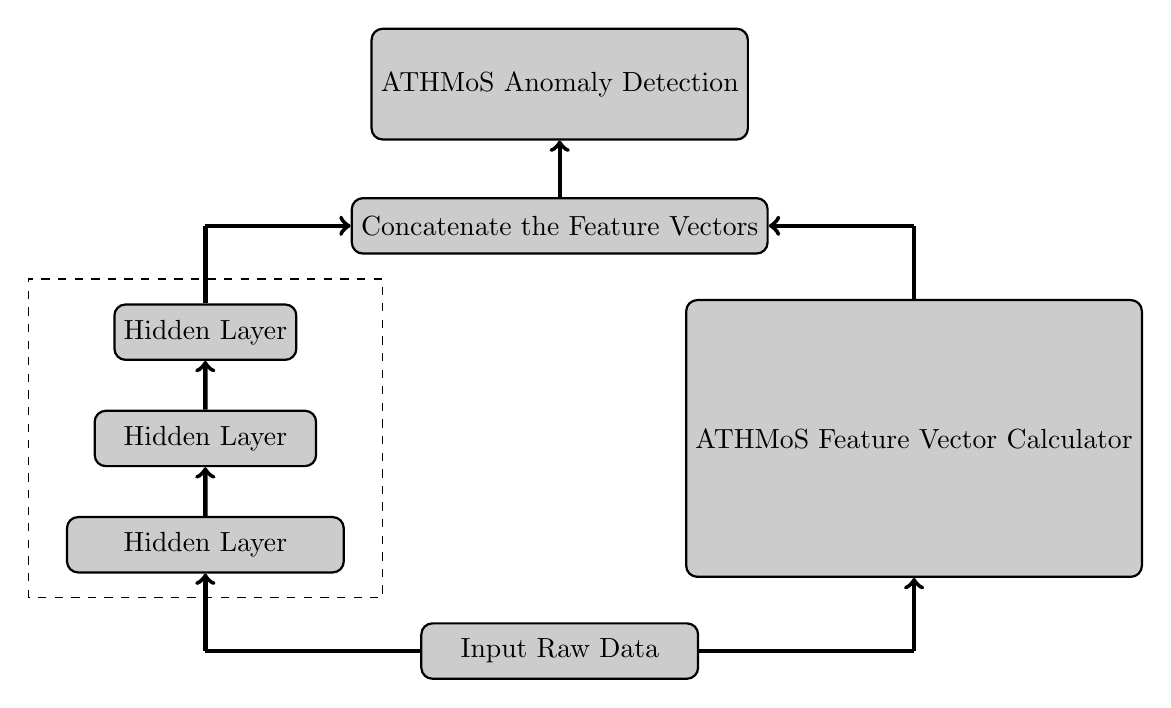
\begin{tikzpicture}[
    block/.style={
      rectangle,
      draw=black,
      thick,
      fill=black!20,
      align=center,
      rounded corners,
      minimum height=2em
    },
    scale=0.9
]

\node[block,minimum height=4em] (aad) at (0,5) {ATHMoS Anomaly Detection};
\node[block] (ctfv) at (0,3) {Concatenate the Feature Vectors};

\draw[->,ultra thick,scale=1.5] (ctfv) -- (aad);

\draw[dashed] (-7.5,-2.25) rectangle (-2.5,2.25);

\node[] (hl) at (-5,3) {};
\node[block, minimum width=6em] (hl3) at (-5,1.5) {Hidden Layer};
\node[block, minimum width=8em] (hl2) at (-5,0) {Hidden Layer};
\node[block, minimum width=10em] (hl1) at (-5,-1.5) {Hidden Layer};

\draw[ultra thick,scale=1.5] (hl3.north) -- (hl.center);
\draw[->,ultra thick,scale=1.5] (hl.center) -- (ctfv.west);
\draw[->,ultra thick,scale=1.5] (hl2) -- (hl3);
\draw[->,ultra thick,scale=1.5] (hl1) -- (hl2);

\node[] (edge) at (5,3) {};
\node[block, minimum height=10em] (afvc) at (5,0) {ATHMoS Feature Vector Calculator};
\draw[ultra thick,scale=1.5] (afvc.north) -- (edge.center);
\draw[->,ultra thick,scale=1.5] (edge.center) -- (ctfv.east);

\node[] (edge1) at (5,-3) {};
\node[] (edge2) at (-5,-3) {};
\node[block, minimum width=10em] (ird) at (0,-3) {Input Raw Data};

\draw[ultra thick,scale=1.5] (ird.east) -- (edge1.center);
\draw[->,ultra thick,scale=1.5] (edge1.center) -- (afvc.south);

\draw[ultra thick,scale=1.5] (ird.west) -- (edge2.center);
\draw[->,ultra thick,scale=1.5] (edge2.center) -- (hl1.south);

\end{tikzpicture}

\caption{\ac{athmos} anomaly detection \cite[p. 8]{athmos}.}
\label{f:athmos_anomaly}
\end{figure}

	\subsection{Automated Telemetry Health Monitoring System (ATHMoS)}
	One example for the anomaly detection technique provided by the authors, was first employed at TET-1 satellite \cite{tet}. Here it was possible to detect an anomaly on a reaction wheel before any boundary detection would have given an alarm \cite[p. 11f]{athmos-sub}.
	
	As this technique is still under development, no hard numbers can be put on the performance. But \ac{athmos} did show that its technique is in general able to work with telemetry in a correct way to predict it in a time frame of 4.5 hours with high accuracy. Along with the distinction between high and low priority anomalies, there is already a benefit regarding satellite health monitoring.

\section{Machine Learning}
\label{c:new_techniques}
New ideas and promising techniques mainly involve \acf{ml}, featuring specifically neural networks. \ac{ml} itself has been in development for many decades. Only in the last decade, computers have become powerful enough to be able to run complex and big neural networks. Hence, using machine learning as a tool for automation and autonomy on \ac{spc} has become an interesting approach for research \cite{ai-dlr-survey}. \newline 
One advantage of \ac{ml} is that it doesn't require as much domain knowledge as statistical methods. Second, statistical methods are not able to process sequential context, which is important when the environment and therefore the data context changes. And third, in general, neural networks can be used to approximate any function, giving them more possible use cases than statistical methods.

As a first step we will here shortly discuss rather simple, but yet powerful, ideas which will later be analysed regarding their performance. These ideas include the \acf{knn}, \acf{aec}, \acf{svm} and \acf{lstm}.

	\subsection{Nearest Neighbour}
	The \ac{knn} algorithm \cite[p. 168ff]{ai-example} is one of the most trivial and simplest ways to divide datasets into groups. It can be used on labelled as well as unlabelled datasets. In the unlabelled case, a margin between groups has to be defined. 
	
\bigbreak

To put the samples into various groups, the distances $\mathbf{D}$ among them has to be calculated:

\begin{equation*}
d_{ij} (P_i, P_j) = \sqrt{(x_i - x_j)^2 + (y_i - y_j)^2}
\end{equation*}	

All points within a certain distance $\left( d_{ij} < \xi \right)$ can form a group and extend this group if they have enough neighbours in their vicinity. If one point has not enough neighbours to form a group of its own, it will be put into a \enquote{noise} group. In figure \ref{f:3_DBSCAN} the execution of a \ac{knn} algorithm is shown. The data has been split into two groups (blue and red) and grey noise points.

\begin{figure}[H]
\centering
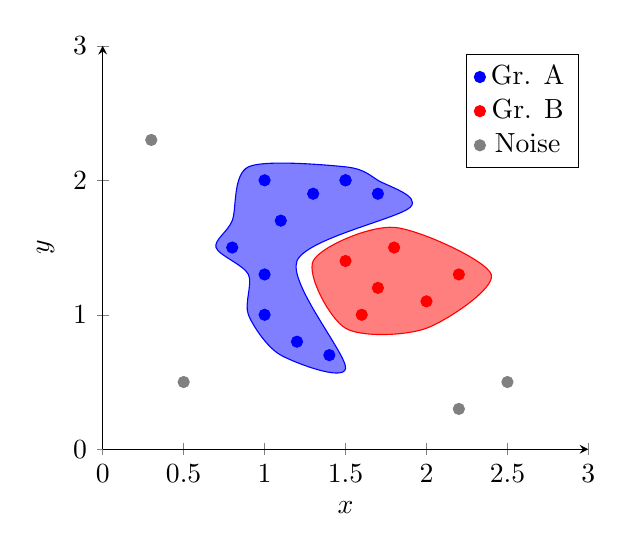
\begin{tikzpicture}
	\begin{axis}[
		xlabel=$x$,
		ylabel=$y$,
		axis x line=bottom,
		axis y line=left,
		ymin=0,
		ymax=3,
		xmin=0,
		xmax=3,
		scale=0.9
]

	\addlegendentry{Gr. A}
	\addplot[only marks, mark=*,color=blue] coordinates {
		(1.4, 0.7) [1]
		(1.2, 0.8) [1]
		(1, 1) [1]
		(1, 1.3) [1]
		(0.8, 1.5) [1]
		(1.1, 1.7) [1]
		(1.3, 1.9)
		(1.5, 2.0)
		(1.5, 2.0)
		(1.0, 2.0)
		(1.7, 1.9)
};

\addlegendentry{Gr. B}
\addplot[only marks, color=red, mark=*] coordinates {
		(1.5, 1.4)
		(1.7, 1.2)
		(1.6, 1.0)
		(2.0, 1.1)
		(2.2, 1.3)
		(1.8, 1.5)
};

\addlegendentry{Noise}
\addplot[only marks, color=gray, mark=*] coordinates {
	(0.5, 0.5)
	(0.3, 2.3)
	(2.5, 0.5)
	(2.2, 0.3)
};

\addplot[smooth cycle, no marks,color=blue,fill=blue, fill opacity=0.5] coordinates {
		(1.5, 0.6)
		(1.1, 0.7)
		(0.9, 1)
		(0.9, 1.3)
		(0.7, 1.5)
		(0.8, 1.7)
		(0.9, 2.1)
		(1.5, 2.1)
		(1.7, 2.0)
		(1.9, 1.8)
		(1.2, 1.4)
};%|- (axis cs:1.2,1.4) -- cycle;

\addplot[smooth cycle, no marks,color=red,fill=red, fill opacity=0.5] coordinates {
		(1.3, 1.4)
		(1.5, 0.9)
		(2.0, 0.9)
		(2.4, 1.3)
		(1.8, 1.65)
};%|- (axis cs:1.8,1.7) -- cycle;

	\end{axis}

\end{tikzpicture}

\caption{k-nearest-neighbour algorithm \enquote{DBSCAN} creates two groups (blue and red) and grey noise points.}
\label{f:3_DBSCAN}
\end{figure}
	
	The computational cost in the standard case is for $N$ samples $\mathcal{O} (N)$. This can be brought down to $\mathcal{O} (\log N)$ with a binary tree and to $\mathcal{O} (1)$ with a hash table \cite[p. 739]{ai-modern}.	

	%TODO Mention that this is not really learning and not supported, therefore we dont use it

	\subsection{Auto-Encoder}
	\acfp{aec} are neural networks for extracting features out of a dataset by the means of encoding the values in a smaller space and decoding it back to the original representation. They have been already used to detect anomalies in various ways \cite{auto-enc-1}\cite{auto-enc-2}\cite{anomaly-basic}. \newline	
	In detail, an \ac{aec} takes the data input vector $\mathbf{x}$, which is then transformed by a trainable weight matrix $\mathbf{W}$ into the hidden layer $\mathbf{h}$. This step is called \enquote{encoding}. The size of $\mathbf{h}$ corresponds to the number of nodes in the layer and is usually smaller than the input in the case of \acp{aec}. The smaller vector $\mathbf{h}$ is then reverse transformed into a vector $\mathbf{y}$ of the same size as the input vector. This step is called \enquote{decoding}. Ideally this should reproduce the previously given input data $\mathbf{x}$. Mathematically written this yields:
	
\begin{align*}
\text{Encoding} & & \mathbf{h} = \mathbf{W}_1\cdot \mathbf{x} \\
\text{Decoding} & & \mathbf{y} = \mathbf{W}_2\cdot \mathbf{h} \\
\end{align*}
	
	This can of course be build with multiple hidden layers. Each layer is then mirrored to give a final output $\mathbf{y}$ equal to the input $\mathbf{x}$. As a general result, the auto-encoder only learns the essential features of the data to recreate the given input. \newline	
	To find anomalies in the end, one has to compare the input vector $\mathbf{x}$ with the output vector $\mathbf{y}$ to calculate any discrepancy.
	
	This basically means, an Auto-Encoder is able to learn a representation of features in a given dataset. Hence it can be used to detect all kinds of features and outliers that were not present before in the particular input from the dataset.
	%Additionally, this method can be used to de-noise the input data.
	The computational cost depends linearly on the number of chosen layers and quadratically on their number of nodes as well as the number of input samples in the given time frame. This totals to a performance of $\mathcal{O} (N^2)$.
	
	\subsection{Support Vector Machines}
	\acfp{svm} \cite[p. 744ff]{ai-modern} are not trivial, but yet quite powerful. They mainly work for separating labelled datasets, but they can also be used in the unsupervised unlabelled case for anomaly detection \cite{one-class-svm}. They work by interpreting every datapoint itself as a vector. Based on that, a boundary line described by a normal vector $\mathbf{w}$ can be drawn to separate these datapoints in a dataset into positive and negative examples:
	
	\begin{equation*}
	y = \mathbf{x}\cdot\mathbf{w} + b = \begin{cases}
	-1 & \text{negative} \\
	\pm 0 & \text{boundary} \\
	+1 & \text{positive} 
	\end{cases}
	\end{equation*}
	
	For datasets that cannot be linearly separated, the dimensionality of the evaluation can be increased with a kernel function. This again can be reduced back with a principal-component-analysis to save computation time. The overall computational cost for finding the boundary line (in training) highly depends on the used optimization algorithm as this is a non-linear optimization problem. For later queries in an already trained network, the cost is linear to the input vector length.
	
	\subsection{Long Short-Term Memory}
	\acfp{lstm} were introduced by Sepp Hochreiter \cite{lstm} out of the need to create a recurrent neural network, that works with learned long-term input as well as recent short-term input. Especially taking into account the chronological order of the various inputs. \newline
	Conventional recurrent networks do suffer from error back propagation with large time delays, where the error gradient would either completely vanish, explode or in some cases even oscillate. This was solved by \enquote{enforcing constant (thus neither exploding nor vanishing) error flow through internal states of special units} \cite[p. 1f]{lstm}. \newline
	In figure \ref{f:lstm} a \ac{lstm} module with its special internal units is shown. Each gate in the module can be thought of as a single neuron. There are the output gate $o_t$, forget gate $f_t$ and input gate $i_t$. In the very middle is the cell $c_t$ memorizing the state. The big S-circles represent the activation functions, like the sigmoid function. The small X-circles are for point-wise multiplication operations.
		
	\acp{lstm} have become interesting only in the recent years with increasing computational power and memory, and the possibility of using huge datasets.
	
	One very important area for \ac{lstm} networks is text and speech recognition. Here the context of a sentence depends on all the sentences said or written before as well as the actual sentence presented. Thus their popularity and use has vastly increased over the recent years.
	
	They have also been proven to be useful in space mission as Kyle Hundman et al. at NASA JPL have shown on two Mars missions \cite{sc-lstm-detection}. With an anomaly detection system built on the basis of an \ac{lstm} they were able to label anomalies in telemetry data in the Mars Science Laboratory (MSL)\footnote{Also known as \enquote{Curiosity}} and the Soil Moisture Active Passive (SMAP) satellite.	
	
	\begin{figure}[htb]
	\centering
	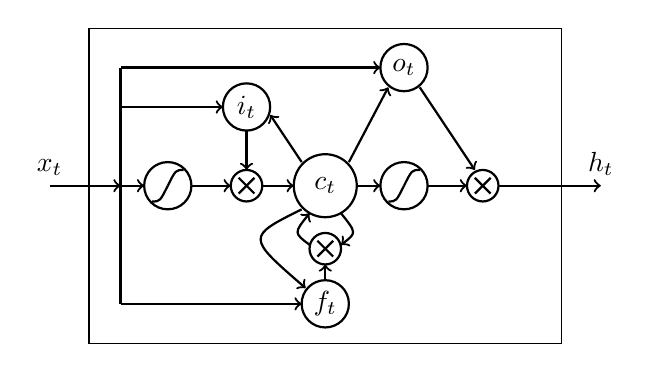
\begin{tikzpicture}

%% Outer box %%
\draw (0,0) rectangle (6,4);

%% Connection arrows %%
% left to right %
\draw[->, thick] (-0.5, 2) -- (0.4, 2) node[pos=0, above] {$x_t$};
\draw[->, thick] (0.4, 2) -- (0.7, 2);

\draw[->, thick] (1.3, 2) -- (1.8, 2);
\draw[->, thick] (2.2, 2) -- (2.6, 2);

\draw[->, thick] (3.4, 2) -- (3.7, 2);
\draw[->, thick] (4.3, 2) -- (4.8, 2);

\draw[->, thick] (5.2, 2) -- (6.5, 2) node[pos=1, above] {$h_t$};

% interconnection %
\draw[thick] (0.4, 3.5) -- (0.4, 0.5);
\draw[thick,->] (0.4, 3.5) -- (3.7, 3.5);
\draw[thick,->] (0.4, 0.5) -- (2.7, 0.5);
\draw[thick,->] (0.4, 3) -- (1.7, 3);

\draw[thick,->] (2, 2.7) -- (2, 2.2);
\draw[thick,->] (2.7, 2.3) -- (2.3, 2.9);
\draw[thick,->] (3.3, 2.3) -- (3.8, 3.25);

\draw[thick,->] (4.2, 3.25) -- (4.9, 2.2);

\draw[thick,->] (3, 0.8) -- (3, 1);

\draw[thick,->] (2.7, 1.7) .. controls (2, 1.35) .. (2.75, 0.7);

\draw[thick,->] (2.8, 1.25) .. controls (2.6, 1.4) .. (2.8, 1.65);
\draw[thick,->] (3.2, 1.65) .. controls (3.4, 1.4) .. (3.2, 1.25);

%% Nodes %%
% Sigmoid left %
\draw[thick] (1, 2) circle (0.3);
\draw[thick] (0.8, 1.8) .. controls (0.9, 1.8) .. (1, 2);
\draw[thick] (1, 2) .. controls (1.1, 2.2) .. (1.2, 2.2);

% Multiplication left %
\draw[thick] (2, 2) circle (0.2);
\draw[thick] (1.9, 1.9) -- (2.1, 2.1);
\draw[thick] (2.1, 1.9) -- (1.9, 2.1);

\draw[thick] (3,2) circle(0.4) node {$c_t$};

% Sigmoid right %
\draw[thick] (4, 2) circle (0.3);
\draw[thick] (3.8, 1.8) .. controls (3.9, 1.8) .. (4, 2);
\draw[thick] (4, 2) .. controls (4.1, 2.2) .. (4.2, 2.2);

% Multiplication right %
\draw[thick] (5, 2) circle (0.2);
\draw[thick] (4.9, 1.9) -- (5.1, 2.1);
\draw[thick] (5.1, 1.9) -- (4.9, 2.1);

% input gate %
\draw[thick] (2, 3) circle (0.3) node {$i_t$};

% output gate %
\draw[thick] (4, 3.5) circle (0.3) node {$o_t$};

% forget gate %
\draw[thick] (3, 0.5) circle (0.3) node {$f_t$};
\draw[thick] (3, 1.2) circle (0.2);
\draw[thick] (2.9, 1.1) -- (3.1, 1.3);
\draw[thick] (3.1, 1.1) -- (2.9, 1.3);

\end{tikzpicture}

	\caption{Structure of an \ac{lstm} module. The data $\mathbf{x}_t$ propagates through activation functions (S-circle), is convoluted (X-circle) and gets offset against the internal gates ($i_t$, $o_t$ and $f_t$) to the output $\mathbf{h}_t$.}
	\label{f:lstm}
	\end{figure}

	In contrast to \acp{svm} as well as basic neural networks, \acp{lstm} can be used to either categorize or predict future output, depending on the last layer. Hence it can be used to input telemetry data and make future predictions including past and recent changes. As a result, these predictions can be tested against simple boundaries to check if a value is about to cross the limit in the near future.

\chapter{Anomaly Detection and Techniques - A Deeper Look}
\label{c:selection}
To get some first estimations and results, a closer look upon the described techniques from chapter \ref{c:new_techniques} is taken. As all techniques have similar complexity and are used in their most simple version, the computational power is not investigated at this point. Instead their error rates of detecting anomalies in given datasets will be analysed. Hence some datasets are created and analysed by these techniques and algorithms. All algorithms are provided by special libraries and are not implemented from scratch.

First, the used programming library Tensorflow \cite{tf-web} is described, which provides the platform for all the used techniques. Second, the generation and configuration of the training set as well as the validation set will be discussed. With these two things at hand, three machine learning techniques will be analysed: \ac{aec}, \ac{svm} and \ac{lstm}. Unfortunately the \ac{knn} is not supported by tensorflow, thus it has to be left out in the evaluation.

\section{Tensorflow}
To focus more on the techniques themselves and less on the development of specific algorithms, the fully integrated machine learning library Tensorflow \cite{tf-web} is used. It is written in C++ with Python and C++ API. As the models are written in Python scripts, every technique shown in the following can be easily referenced, adapted, modified and extended in further investigations.

The neural networks being built and used consist only of a few layers to keep them as simple as the generated anomaly test cases.

	\subsection{TF-Lite Models}
	Tensorflow allows the export of trained models of neural networks of any kind. These models can then be modified to be \enquote{tf-lite} models. The Lite version of Tensorflow is made to be lightweight, so they can be executed on systems with low resources and computing power, like a System-on-Chip used in a satellite. To execute the exported models on a different platform, two parts are needed. One is the code library to execute tf-lite models. And the second is of course the model itself, to describe the trained neural network. These models are in fact small in their size, but unfortunately they are restricted in their functionality in some parts. Thus some modification might be necessary in order to export them onto a different system later on. 

	It has to be noted, that the Tensorflow code library itself takes a lot of permanent storage, relative to the tf-lite models. But as the code library stays constant, while the only exchangeable parts are the models, this is considered not much of a problem.
	
\section{Generating Training and Validation Sets}
In chapter \ref{c:anomaly_definition}, we defined three cases of anomalies (slope, pulse and sine). In the following we will first define the parameters and shape of the general dataset used for training and validation. Respectively a look into the anomalous datasets and their parameters is taken.

For all anomalies put into the training set and validation set it holds, that their effect always takes half an orbit period ($t_a=50$ minutes) and that they start on random positions $t_0$ within one orbit. For both training and validation, the anomaly parameters are equal and every dataset holds only one type of anomaly. Their parameters are then changed with every new set of training and validation datasets. \newline
Regarding the amount of anomalies, the training set contains 1\% and the valdiationset 10\% anomalous orbits. The anomalies in the training set are put in to simulate an unclean dataset, which might be a very likely case, as we are assuming the learning is done during the mission. The bigger amount of anomalies in the validation set is set to increase confidence in the evaluation results. \newline
Both datasets have labels for normal and anomalous data. These labels are strictly used for the validation as we are focusing on unsupervised learning.

	\subsection{Training Set Definition}
	The training set is based on a normalized arbitrary sensor varying over one orbit period as can be seen in figure \ref{f:trainingset}. The data starts at $x(t=0) = 0.5$ and has its maximum at $x(t=50) = 1.0$. The timesteps are based on a LEO satellite with an orbital period of 100 minutes and one datapoint per minute. Additionally Gaussian white noise is added with a standard deviation of $\sigma = 0.05$. \newline
	One could interpret the data-curve for example as a temperature or current sensor increasing its value up to 100\% in the vicinity of the sun and reducing its value to 50\% during the eclipse.
	
	Before training with the model, the datasets are scaled down to never exceed any value above one. The reason is that certain activation functions only produce values between $\pm 1$, thus making it impossible to learn representations with greater values.

	\begin{figure}[htb]
	\centering
	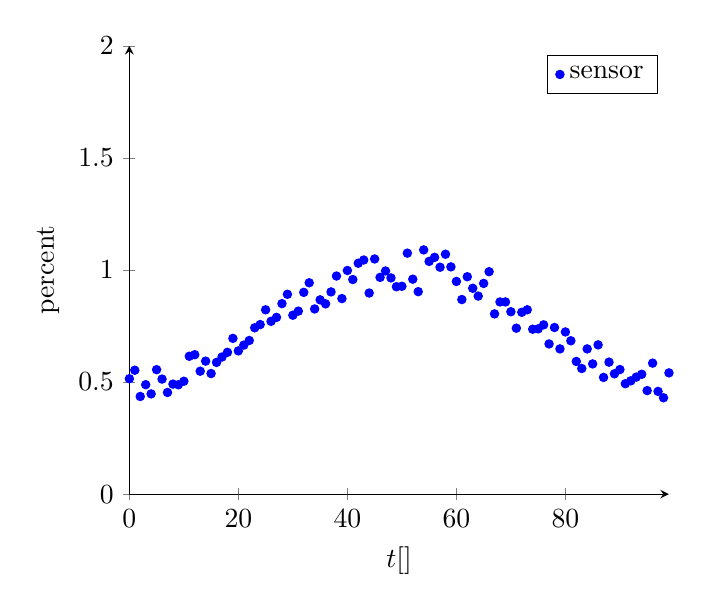
\begin{tikzpicture}
	\begin{axis}[
		xlabel={$t [\SI{}{\second}]$},
		ylabel=percent,
		axis x line=bottom,
		axis y line=left,
		ymin=0,
		ymax=2,
]
	\addplot[only marks, mark size=1.5pt, color=blue, mark=*] plot coordinates {
		(0, 0.5148135091211293)
		(1, 0.5527093648118251)
		(2, 0.4356343885678995)
		(3, 0.4882032268433586)
		(4, 0.4471494697092668)
		(5, 0.5553187915294323)
		(6, 0.5132645572790916)
		(7, 0.4535454087445306)
		(8, 0.4908001359361774)
		(9, 0.4878674913871922)
		(10, 0.503646901781738)
		(11, 0.6150344861440005)
		(12, 0.6219939091500365)
		(13, 0.5484300369146085)
		(14, 0.593319579970499)
		(15, 0.5379975510933108)
		(16, 0.5876450497451683)
		(17, 0.6117143740348091)
		(18, 0.6326219983151554)
		(19, 0.6948684210767105)
		(20, 0.6390364845662206)
		(21, 0.6647360064235809)
		(22, 0.6854067386092852)
		(23, 0.7420813326586236)
		(24, 0.7564828891390465)
		(25, 0.8223075140225933)
		(26, 0.770936328002129)
		(27, 0.7885484201106624)
		(28, 0.8499170162245753)
		(29, 0.89155025729968)
		(30, 0.7981563812065633)
		(31, 0.8164144831350859)
		(32, 0.9001691909305536)
		(33, 0.9428892442550432)
		(34, 0.826198653919079)
		(35, 0.8667604146849139)
		(36, 0.8489087203931843)
		(37, 0.9021208512591392)
		(38, 0.97300936952514)
		(39, 0.8723374403687617)
		(40, 0.9975757096094338)
		(41, 0.9574047933689164)
		(42, 1.030177214599312)
		(43, 1.044449356733221)
		(44, 0.8971423496204484)
		(45, 1.0490300296509223)
		(46, 0.9670163527834132)
		(47, 0.9954300773452464)
		(48, 0.9645744210008248)
		(49, 0.9252106896046788)
		(50, 0.9273240724068952)
		(51, 1.0750236178020676)
		(52, 0.9588681171409954)
		(53, 0.9031929348667098)
		(54, 1.0895479445923888)
		(55, 1.0382244922523924)
		(56, 1.0563745056516842)
		(57, 1.0122847775820645)
		(58, 1.07026537730031)
		(59, 1.0138144834148135)
		(60, 0.9488640434142104)
		(61, 0.868075775460962)
		(62, 0.9698542592842236)
		(63, 0.9183461746492512)
		(64, 0.8835771442261959)
		(65, 0.9400315855036612)
		(66, 0.9923618259350392)
		(67, 0.8041383950707575)
		(68, 0.857304624404517)
		(69, 0.8574620196881786)
		(70, 0.8136329016261772)
		(71, 0.7403006998651073)
		(72, 0.8112125293922191)
		(73, 0.8224310010504874)
		(74, 0.7358001805178063)
		(75, 0.7373332481110552)
		(76, 0.7551414742440595)
		(77, 0.6700339655252157)
		(78, 0.7434164751085204)
		(79, 0.6479706074024576)
		(80, 0.7235317369281178)
		(81, 0.6841663812000243)
		(82, 0.5918532162104058)
		(83, 0.5604967812412956)
		(84, 0.6478597306902443)
		(85, 0.5809575710083209)
		(86, 0.665846100350215)
		(87, 0.5207151045744567)
		(88, 0.588862217051322)
		(89, 0.5368171008431317)
		(90, 0.5557515103067818)
		(91, 0.4925344144657987)
		(92, 0.5054579884686016)
		(93, 0.5221670750434217)
		(94, 0.5346606972935559)
		(95, 0.4619341524206037)
		(96, 0.5843752073820241)
		(97, 0.4582424930128891)
		(98, 0.4299032208781361)
		(99, 0.5408565684086196)
	};
	\addlegendentry{sensor}
	\end{axis}
\end{tikzpicture}

	\caption{Arbitrary satellite sensor data over 100 minutes with 1 datapoint per minute.}
	\label{f:trainingset}
	\end{figure}

	\subsection{Slopeset}
	The slope represents a drifting sensor that shifts the original data $x(t)$ permanently for the rest of the respective orbital period:
	
	\begin{equation}
	\tilde{x}(t) = x(t) + \begin{cases} 
	0 & t < t_0 \\
	(t - t_0) \cdot m & t_0 < t < (t_a+t_0)\\ 
	t_a \cdot m & (t_a+t_0) < t \\
	\end{cases}
	\end{equation}

	In figure \ref{f:slopeset} an anomalous drift with a slope of $m=0.01$ is represented. This slope will be varied to test the anomaly detection.	
	
	\begin{figure}[htb]
	\centering
	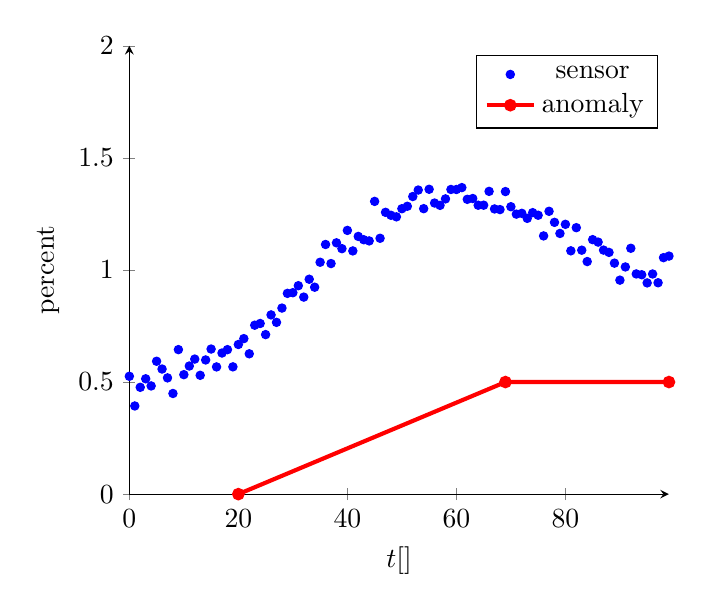
\begin{tikzpicture}
	\begin{axis}[
		xlabel={$t [\SI{}{\second}]$},
		ylabel=percent,
		axis x line=bottom,
		axis y line=left,
		ymin=0,
		ymax=2,
]
	\addplot[only marks, mark size=1.5, color=blue, mark=*] plot coordinates {
		(0, 0.5257202519531616)
		(1, 0.3933064193308462)
		(2, 0.4765423628106863)
		(3, 0.514575080730433)
		(4, 0.4826769821214909)
		(5, 0.5927763086748179)
		(6, 0.5580948882384427)
		(7, 0.5186385660530217)
		(8, 0.4489956396259226)
		(9, 0.6446633100438279)
		(10, 0.5329859806915088)
		(11, 0.5715207197711392)
		(12, 0.602487773377396)
		(13, 0.5301164130763625)
		(14, 0.5985586861225247)
		(15, 0.647282848047128)
		(16, 0.5675534318032193)
		(17, 0.629565261386642)
		(18, 0.6445913369978785)
		(19, 0.5678837088455235)
		(20, 0.6675753317327269)
		(21, 0.6937257051352685)
		(22, 0.6260782607411427)
		(23, 0.7536336104954197)
		(24, 0.7612410223035029)
		(25, 0.711706279092276)
		(26, 0.7995808444792601)
		(27, 0.7663082632517743)
		(28, 0.8300231388299534)
		(29, 0.8956601980213661)
		(30, 0.898681570178228)
		(31, 0.929815218202781)
		(32, 0.8789957664955762)
		(33, 0.9586765920228691)
		(34, 0.923074293486429)
		(35, 1.0344699764375596)
		(36, 1.1137456006918842)
		(37, 1.0286324904345716)
		(38, 1.121179726643802)
		(39, 1.0950945866263622)
		(40, 1.176524365664683)
		(41, 1.0849758359686614)
		(42, 1.1496873585509666)
		(43, 1.134916535749869)
		(44, 1.1296160332215543)
		(45, 1.30599633362797)
		(46, 1.1414630861714743)
		(47, 1.2571562073431812)
		(48, 1.2439985506093014)
		(49, 1.237056948699477)
		(50, 1.2733084446356864)
		(51, 1.2841665085962015)
		(52, 1.3276389265869846)
		(53, 1.3565383660775645)
		(54, 1.2735118732888109)
		(55, 1.3600115927211054)
		(56, 1.2986522290659923)
		(57, 1.2882463480507629)
		(58, 1.317094437073952)
		(59, 1.3591359322055077)
		(60, 1.3590085569928254)
		(61, 1.367468361788795)
		(62, 1.31508168118879)
		(63, 1.3188337572113271)
		(64, 1.2888414736032452)
		(65, 1.2889812462206034)
		(66, 1.3506904512731208)
		(67, 1.27226388350395)
		(68, 1.2693901296688683)
		(69, 1.3497402658033824)
		(70, 1.2821222343086116)
		(71, 1.2491197079127203)
		(72, 1.252651112685624)
		(73, 1.2303388429758226)
		(74, 1.255702174185061)
		(75, 1.2441434558899065)
		(76, 1.15199447619792)
		(77, 1.2617620666991711)
		(78, 1.2124762755525378)
		(79, 1.1629171888096446)
		(80, 1.2036451813972604)
		(81, 1.0854297430524005)
		(82, 1.1886944737051648)
		(83, 1.0882598303661637)
		(84, 1.03759557204201)
		(85, 1.1352745472810162)
		(86, 1.1243775860836926)
		(87, 1.088625261757732)
		(88, 1.078429058779722)
		(89, 1.030418359260421)
		(90, 0.954589459971597)
		(91, 1.013484973606949)
		(92, 1.0967764198561851)
		(93, 0.9823307865562344)
		(94, 0.9787176692765628)
		(95, 0.9423111544572428)
		(96, 0.982070073991782)
		(97, 0.9429599959006084)
		(98, 1.054922303873196)
		(99, 1.0619363850751065)
	};	
	\addplot[line width=1.5pt, mark size=1.5pt, color=red, mark=*] plot coordinates {
	(20, 0.0)	
	(69, 0.5)
	(99, 0.5)
	};
	\addlegendentry{sensor}
	\addlegendentry{anomaly}
	\end{axis}
\end{tikzpicture}

	\caption{Arbitrary satellite sensor data over 100 minutes with 1 datapoint per minute with a slope anomaly of $m=0.01$.}
	\label{f:slopeset}
	\end{figure}
	
	\subsection{Pulseset}
	The pulse represents a single event effect which might offset the data temporary or permanently. Such an effect can cause a destruction of a component in the worst case. In the best case the faulty sensor may actually be recovered. 
	
	In this case, only a temporary non-destructive pulse is assumed, as this shape is harder to detect than a permanently offset curve. The anomaly is described by:
	
	\begin{equation}
	\tilde{x}(t) = x(t) \cdot \begin{cases} 
	h & t_0 < t < (t_a+t_0)\\ 
	1 & \text{other} \\
	\end{cases}	
	\end{equation}
	
	The pulse gets multiplied instead of added onto the values to better align with the current values on the original curve. In figure \ref{f:pulseset} an anomalous pulse with the height $h=1.5$ is represented. The height of the pulse will be varied to test the anomaly detection.

	\begin{figure}[htb]
	\centering
	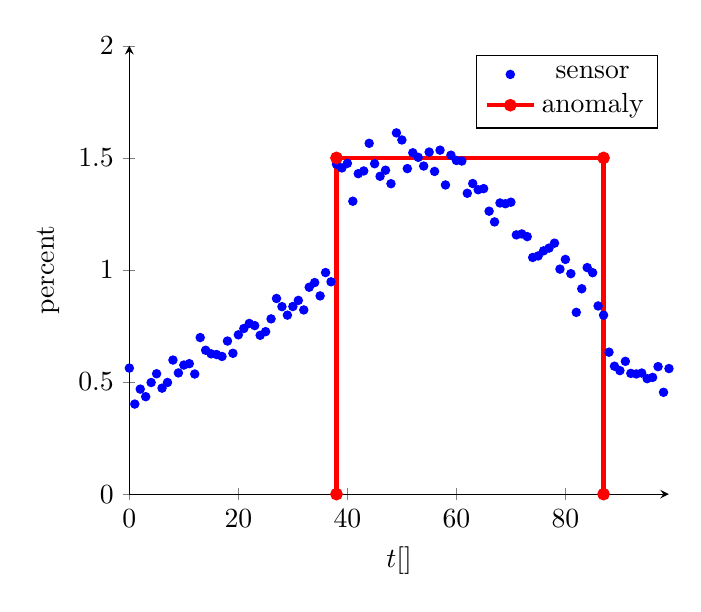
\begin{tikzpicture}
	\begin{axis}[
		xlabel={$t [\SI{}{\second}]$},
		ylabel=percent,
		axis x line=bottom,
		axis y line=left,
		ymin=0,
		ymax=2,
]
	\addplot[only marks, mark size=1.5, color=blue, mark=*] plot coordinates {
		(0, 0.5622681255888685)
		(1, 0.4018484176094724)
		(2, 0.468539007627844)
		(3, 0.4346494223779653)
		(4, 0.4978784570823389)
		(5, 0.5369804910433361)
		(6, 0.4728006879373315)
		(7, 0.4980667892486829)
		(8, 0.5981732065691774)
		(9, 0.5406475645957558)
		(10, 0.5758970004919037)
		(11, 0.5820192466705968)
		(12, 0.5358814379228652)
		(13, 0.6985123457380722)
		(14, 0.6418230691511462)
		(15, 0.6259568634991284)
		(16, 0.6228037495559587)
		(17, 0.6142382050392389)
		(18, 0.6829744918718758)
		(19, 0.6283544026585022)
		(20, 0.7106970383550277)
		(21, 0.7387633572763191)
		(22, 0.7613516325817288)
		(23, 0.7518259428929189)
		(24, 0.7085304833469191)
		(25, 0.7248916181056512)
		(26, 0.7818339897820638)
		(27, 0.8728052695420704)
		(28, 0.8363648257606918)
		(29, 0.798578382982168)
		(30, 0.8369787265765458)
		(31, 0.8642619011492502)
		(32, 0.8217206778146873)
		(33, 0.9229330326870384)
		(34, 0.9438318609940126)
		(35, 0.884290851371344)
		(36, 0.9884099128558124)
		(37, 0.9472086834843008)
		(38, 1.471853350803487)
		(39, 1.4551641478178805)
		(40, 1.4757124032678597)
		(41, 1.306727213897842)
		(42, 1.42966014896879)
		(43, 1.4415885000587778)
		(44, 1.5650498459900015)
		(45, 1.4739488414455062)
		(46, 1.417947761481765)
		(47, 1.4450155271319116)
		(48, 1.3847903197379563)
		(49, 1.6114751130208167)
		(50, 1.5798710730089405)
		(51, 1.4522208486083072)
		(52, 1.522777221034119)
		(53, 1.5025269511446142)
		(54, 1.4637374176823832)
		(55, 1.5259716170145772)
		(56, 1.4396395877696049)
		(57, 1.5345736716183676)
		(58, 1.379217889855051)
		(59, 1.5121303474940588)
		(60, 1.4885356534206915)
		(61, 1.486039772970771)
		(62, 1.3422151925316064)
		(63, 1.3856347694561453)
		(64, 1.3579218007071867)
		(65, 1.3629474402397117)
		(66, 1.262192683391942)
		(67, 1.214390004115027)
		(68, 1.2988363035721806)
		(69, 1.295562163790969)
		(70, 1.3022986427123642)
		(71, 1.1564995456286935)
		(72, 1.1607266623433263)
		(73, 1.1488209048019624)
		(74, 1.055722045560718)
		(75, 1.0626395333526133)
		(76, 1.085452079010005)
		(77, 1.0976302853770157)
		(78, 1.1196388278104767)
		(79, 1.0038123805549373)
		(80, 1.047022344086964)
		(81, 0.9834891102206752)
		(82, 0.8108537092128778)
		(83, 0.91611121401388)
		(84, 1.0106004534103308)
		(85, 0.9878357379686592)
		(86, 0.8395357967308059)
		(87, 0.7984144669733708)
		(88, 0.633296672803493)
		(89, 0.5707306169302587)
		(90, 0.5510750847565071)
		(91, 0.592365635376908)
		(92, 0.5387179602616414)
		(93, 0.5360967358732206)
		(94, 0.540274363763101)
		(95, 0.5151774336847359)
		(96, 0.5206740294922417)
		(97, 0.5687780360671054)
		(98, 0.4542974576912108)
		(99, 0.5602258913233213)
	};
	\addplot[line width=1.5pt, mark size=1.5pt, color=red, mark=*] plot coordinates {
	(38,0)	
	(38, 1.5)
	(87, 1.5)
	(87,0)	
	};
	\addlegendentry{sensor}
	\addlegendentry{anomaly}
	\end{axis}
\end{tikzpicture}

	\caption{Arbitrary satellite sensor data over 100 minutes with 1 datapoint per minute with a pulse anomaly of $h=1.5$.}
	\label{f:pulseset}
	\end{figure}
		
	\subsection{Sineset}
	The sine represents an oscillating sensor value which can have many different causes. But the effect may be severe as the oscillation might apparently cancel out in averaging or slow measurements.
	
	Again, only a temporary anomaly is assumed. The sine gets added onto the original curve for alignment:
	
	\begin{equation}
	\tilde{x}(t) = x(t) + \begin{cases} 
	a\cdot \sin \left( 2 \pi\cdot \frac{t - t_0}{T} \right) & t_0 < t < (t_a+t_0)\\ 
	0 & \text{other} \\
	\end{cases}	
	\end{equation}
	
	In figure \ref{f:sineset} an anomalous sine with the amplitude of $a=0.1$ and a period of $T=10$ is represented. The amplitude is varied to test the anomaly detection. The period is an integer part of the anomaly length $t_a$.

	\begin{figure}[htb]
	\centering
	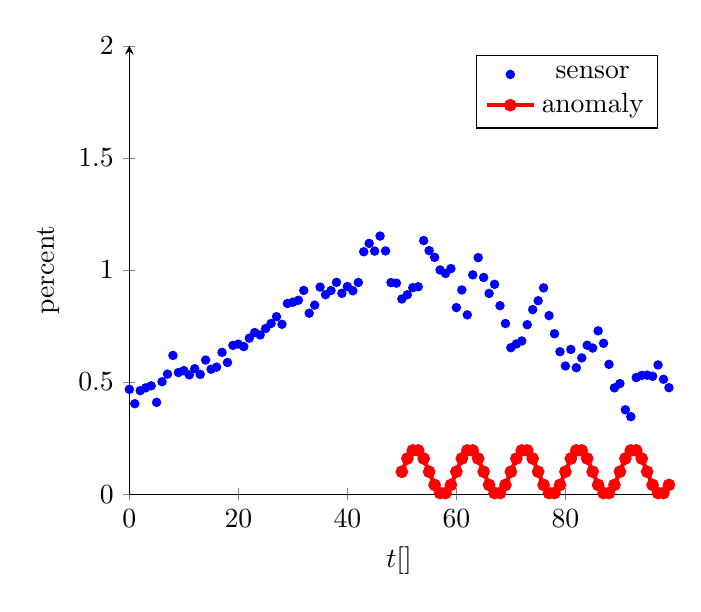
\begin{tikzpicture}
	\begin{axis}[
		xlabel={$t [\SI{}{\second}]$},
		ylabel=percent,
		axis x line=bottom,
		axis y line=left,
		ymin=0,
		ymax=2,
]
	\addplot[only marks, mark size=1.5pt, color=blue, mark=*] plot coordinates {
		(0, 0.4675710930720688)
		(1, 0.4035288384420797)
		(2, 0.4614994617543668)
		(3, 0.4741826206690595)
		(4, 0.4833636250440074)
		(5, 0.4094383213712222)
		(6, 0.50149094046001)
		(7, 0.5354831493731601)
		(8, 0.6187755077491178)
		(9, 0.542344304412583)
		(10, 0.5508732150855068)
		(11, 0.5320931867758759)
		(12, 0.559653593307129)
		(13, 0.5339395471706596)
		(14, 0.5981107538336488)
		(15, 0.5572133561652093)
		(16, 0.5664987356334859)
		(17, 0.6324855895660142)
		(18, 0.5872022144578057)
		(19, 0.6634890035108082)
		(20, 0.6692050431485325)
		(21, 0.6582144349087283)
		(22, 0.6958281459247948)
		(23, 0.7208034426364467)
		(24, 0.7101306621856089)
		(25, 0.7387057972318111)
		(26, 0.7612088897207089)
		(27, 0.7914799733472769)
		(28, 0.7577919279220948)
		(29, 0.8505524975227555)
		(30, 0.8563159498771499)
		(31, 0.8648936229685991)
		(32, 0.9086648675675624)
		(33, 0.8071646998451336)
		(34, 0.8432449971193889)
		(35, 0.9237126615689984)
		(36, 0.8899132110047788)
		(37, 0.908340231208818)
		(38, 0.9450501046375054)
		(39, 0.8959981381306558)
		(40, 0.925945783447266)
		(41, 0.9073053735460924)
		(42, 0.9440756484326074)
		(43, 1.0813841424338937)
		(44, 1.1185867916060055)
		(45, 1.084207526935188)
		(46, 1.1512711334319354)
		(47, 1.085020953933012)
		(48, 0.9438495063804538)
		(49, 0.9412338104671244)
		(50, 0.870473771574796)
		(51, 0.8894045880114038)
		(52, 0.9209297945039918)
		(53, 0.9251794570707824)
		(54, 1.1312347209956808)
		(55, 1.086388063537855)
		(56, 1.056141698612158)
		(57, 0.9999754123748686)
		(58, 0.9842802413972164)
		(59, 1.006236151553452)
		(60, 0.8322287014524513)
		(61, 0.9108820853239074)
		(62, 0.7996822536374895)
		(63, 0.978290658944277)
		(64, 1.055107679397448)
		(65, 0.9665039821190108)
		(66, 0.895378992066291)
		(67, 0.9359424873924602)
		(68, 0.8407571588452414)
		(69, 0.7611689886354749)
		(70, 0.653279449175096)
		(71, 0.6698868550702144)
		(72, 0.6832408162687862)
		(73, 0.7558265917207679)
		(74, 0.8232249957379556)
		(75, 0.8627145122568253)
		(76, 0.9200452478952312)
		(77, 0.7964714969045936)
		(78, 0.715483377729346)
		(79, 0.6352946027855869)
		(80, 0.5716298021591403)
		(81, 0.6454422831205586)
		(82, 0.5640832188799343)
		(83, 0.6076782595238305)
		(84, 0.6641849212298528)
		(85, 0.65170372756007)
		(86, 0.7284030983671312)
		(87, 0.6729056096993876)
		(88, 0.5790123981700747)
		(89, 0.4741078650301549)
		(90, 0.4930747376159831)
		(91, 0.376191666455661)
		(92, 0.3454441535771184)
		(93, 0.5201426407838525)
		(94, 0.5298863316224143)
		(95, 0.530793936638022)
		(96, 0.5259402317831131)
		(97, 0.5762361607310418)
		(98, 0.5124108093224641)
		(99, 0.4750412108932678)
	};
	\addplot[line width=1.5pt, mark size=1.5pt, color=red, mark=*] plot coordinates {
(50, 0.1)
(51, 0.15877852522924732)
(52, 0.19510565162951538)
(53, 0.19510565162951538)
(54, 0.15877852522924735)
(55, 0.10000000000000002)
(56, 0.0412214747707527)
(57, 0.00489434837048465)
(58, 0.004894348370484636)
(59, 0.041221474770752664)
(60, 0.09999999999999998)
(61, 0.15877852522924724)
(62, 0.19510565162951538)
(63, 0.19510565162951538)
(64, 0.15877852522924735)
(65, 0.10000000000000005)
(66, 0.04122147477075272)
(67, 0.0048943483704846635)
(68, 0.004894348370484622)
(69, 0.04122147477075266)
(70, 0.09999999999999995)
(71, 0.1587785252292473)
(72, 0.1951056516295153)
(73, 0.19510565162951538)
(74, 0.15877852522924737)
(75, 0.10000000000000006)
(76, 0.04122147477075275)
(77, 0.0048943483704846635)
(78, 0.004894348370484622)
(79, 0.041221474770752636)
(80, 0.09999999999999994)
(81, 0.15877852522924726)
(82, 0.19510565162951535)
(83, 0.1951056516295154)
(84, 0.1587785252292474)
(85, 0.10000000000000009)
(86, 0.041221474770752754)
(87, 0.0048943483704846635)
(88, 0.004894348370484608)
(89, 0.04122147477075261)
(90, 0.09999999999999991)
(91, 0.15877852522924696)
(92, 0.19510565162951535)
(93, 0.1951056516295154)
(94, 0.1587785252292477)
(95, 0.10000000000000012)
(96, 0.041221474770752775)
(97, 0.004894348370484566)
(98, 0.004894348370484608)
(99, 0.0412214747707523)
	};
	\addlegendentry{sensor}
	\addlegendentry{anomaly}
	\end{axis}
\end{tikzpicture}

	\caption{Arbitrary satellite sensor data over 100 minutes with 1 datapoint per minute with sine anomaly of $a=0.1$ and $T=10$.}
	\label{f:sineset}
	\end{figure}

\section{Evaluation of Anomaly Detection Techniques}
To test and evaluate the discussed anomaly detection techniques, they are first trained accordingly with a training set (1\% anomalies) and then queried with a validation set (10\% anomalies). As a reference, one year of operation is taken, leading to a total of $N = 5256$ orbits within each dataset. A specific orbit will be referenced with an index $i = 1, \hdots, N$. With a trained model at hand, the validation set is fed in. The technique shall now detect and report every identified anomaly. These results are then compared to the actual labels of the corresponding validation set to check if the detection is working correctly. \newline
For an overall comparison the effective detection rate is measured. This includes the percentage of detected anomalies (true-positive-rate) and the percentage of miss-categorizations (false-positive-rate). 

First the discussed techniques are set up in a way to give the best result with the least amount of computation power, in order to achieve a realistic test-scenario. This includes for example the number of nodes, layers and training epochs. \newline
Furthermore, the decision boundary between normal and anomalous data is set to allow on average only one miss-categorization (false-positive) per month, so 12 miss-categorizations per dataset or respectively 0.23\%.

In the following the individual algorithms are first examined and set up. And in the end, a comparison between each technique in the respective anomaly domain is drawn.

	\bigbreak
	
	The used ranges for the training sets as well as validation sets can be found in the following table \ref{t:parameter-range}:
	
	\begin{table}[htb]
	\centering
	\begin{tabular}{llll}
	\toprule
	Parameter	& Start		& Stop		& Steps		\\ \midrule
	Slope $m$	& 0.0001	& 0.0051	& 0.0001	\\
	Pulse $h$	& 1.004		& 1.204		& 0.004		\\
	Sine $a$	& 0.003		& 0.153		& 0.003		\\ \bottomrule
	\end{tabular}
	\caption{Parameter range for the three anomaly types.}
	\label{t:parameter-range}
	\end{table}

	\subsection{Auto-Encoder}
	The used \ac{aec} has an input and output with the size of the dataset. It has only one hidden layer consisting of 25 nodes. Therefore, only one encoding matrix $\mathbf{W}_e$ and one decoding matrix $\mathbf{W}_d$ are needed. The number of nodes was chosen as a comprise between computing resources and detection quality. The training time it took for convergence was usually 4 to 5 epochs. For more details of the model, see the source code in chapter \ref{c:src_aec}.
	
	To distinguish between normal an anomalous data, the difference between the original curve and the output of the \ac{aec} are compared:
	
	\begin{equation*}
	e_i = \left| \mathbf{x}_i - \mathbf{y}_i \right|
	\end{equation*}
	
	Now a boundary has to be estimated to know if the error $e_i$ indicates an anomaly. This can be done by taking the training set and storing all the errors in a vector $\mathbf{e}$. This vector $\mathbf{e}$ is then sorted for ascending values. Then we have to make two assumption. First that most of our data is not anomalous, for example at least 90\%. Second, that our error $\mathbf{e}$ is a normal distribution, which is the case for the dataset used here. \newline
	With this, one can cut off the lower half of the vector $\mathbf{e}$. This gives a curve with an almost linear slope in the beginning and a exponential ascend in the end. From these two parts on the curve two linear fits can be made. One following the linear part and one the exponential ascend. To find the cut off between linear and exponential part, the intersection of the to linear fits is calculated. This cut off value $e_i$ is then used as the boundary. The visualisation of the evaluation curves can be seen in figure \ref{f:cutoff}. \newline
	Additionally this processing step could also be used to first prune the data and to repeat the whole process to get a more accurate boundary.
	
	\begin{figure}[htb]
	\centering
	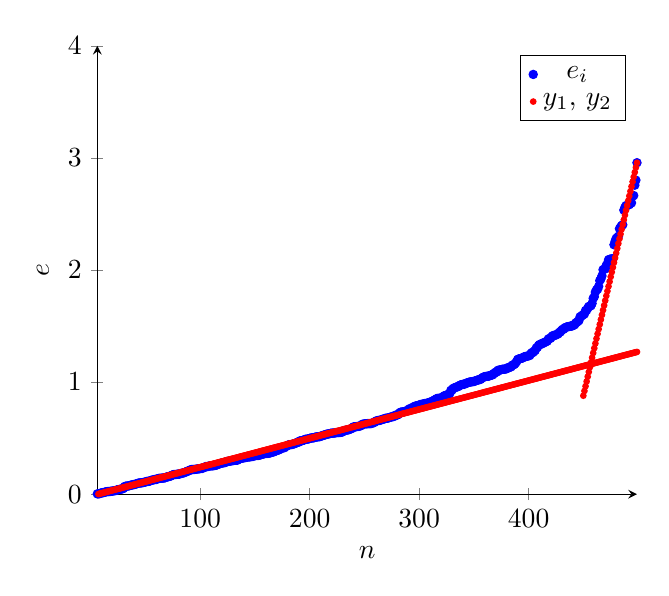
\begin{tikzpicture}
	\begin{axis}[
		xlabel=$n$,
		ylabel=$e$,
		axis x line=bottom,
		axis y line=left,
		ymin=0,
		ymax=4,
]
	\addplot[only marks, mark size=1.5, color=blue, mark=*] plot coordinates {
(0,-0.017073391060067986)
(1,-0.016479882807693212)
(2,-0.015393647220525962)
(3,-0.01392844102566872)
(4,-0.012214478520946164)
(5,-0.0009605735635448366)
(6,0.0023854634423883738)
(7,0.0030761254602199835)
(8,0.003865015745962922)
(9,0.009685925081924326)
(10,0.010874263266593853)
(11,0.0131309115389229)
(12,0.014343385107826965)
(13,0.01815212598944178)
(14,0.020873056676151587)
(15,0.022777295598912214)
(16,0.023224719299402646)
(17,0.02340304597589945)
(18,0.024850611978277152)
(19,0.026366226224690783)
(20,0.027140042800431384)
(21,0.0296194448059916)
(22,0.03087550551012838)
(23,0.032544168519036035)
(24,0.03800956860936971)
(25,0.0397227664935637)
(26,0.041586708267143745)
(27,0.043990676759404865)
(28,0.04557130833049707)
(29,0.04721607254894133)
(30,0.052754978753981996)
(31,0.06800064537800932)
(32,0.07060965946468811)
(33,0.07240691032569)
(34,0.07251111485629104)
(35,0.0742375088709183)
(36,0.07789583476482474)
(37,0.08144222261076248)
(38,0.0815412838337198)
(39,0.08564700283923021)
(40,0.08591869369025322)
(41,0.08886434180461295)
(42,0.0935256061035525)
(43,0.09579176253373356)
(44,0.09958827165502243)
(45,0.09978999851185133)
(46,0.10013923335204936)
(47,0.10220811765742475)
(48,0.10364563145165971)
(49,0.10626966271789698)
(50,0.10829734408893148)
(51,0.11287344487727162)
(52,0.1134543726870243)
(53,0.11401918479584681)
(54,0.11663010751881478)
(55,0.12293129825260932)
(56,0.12437824287252366)
(57,0.12644338288337334)
(58,0.13042718040629683)
(59,0.13094538306493275)
(60,0.13099323003444957)
(61,0.1372502844408006)
(62,0.1396901351214353)
(63,0.1409908308970273)
(64,0.14153122919492037)
(65,0.14308967379916424)
(66,0.1432744225691531)
(67,0.14449661181619045)
(68,0.14611625046452015)
(69,0.15214712160833016)
(70,0.15492531673088633)
(71,0.1554323929291994)
(72,0.1593668906580029)
(73,0.16092678240803823)
(74,0.16748138842316704)
(75,0.1726651909084545)
(76,0.17478823442418556)
(77,0.1751006096706167)
(78,0.1756407173306756)
(79,0.17761930372131932)
(80,0.1783513937298219)
(81,0.17880950668669104)
(82,0.18415108518400425)
(83,0.1843449015560988)
(84,0.18940334855829966)
(85,0.19008692296226898)
(86,0.19372621647137542)
(87,0.1998999991547279)
(88,0.20221155136339455)
(89,0.2079177329998113)
(90,0.2099189033618004)
(91,0.21661593037091942)
(92,0.21953988081753134)
(93,0.21970053530351466)
(94,0.22005090446936493)
(95,0.22022335262965842)
(96,0.22222218637785324)
(97,0.22362683549533205)
(98,0.225811179570568)
(99,0.22596792047043404)
(100,0.22823579142078448)
(101,0.22996171451488642)
(102,0.23028081278207754)
(103,0.23648556649104582)
(104,0.23902915062881339)
(105,0.24525632368644681)
(106,0.24623155823913773)
(107,0.24641032624486814)
(108,0.25084044049864296)
(109,0.2521668380025177)
(110,0.25247203301048926)
(111,0.2531580929029765)
(112,0.2533781155470784)
(113,0.25598101710103527)
(114,0.25715911341834374)
(115,0.2598132704023236)
(116,0.2643744114601719)
(117,0.2691977535833011)
(118,0.27130706286822975)
(119,0.2750815468413491)
(120,0.27818454984321545)
(121,0.27949627615671785)
(122,0.2807370756536759)
(123,0.2824090599944281)
(124,0.2910182306171525)
(125,0.2914480127772875)
(126,0.29331941366498754)
(127,0.2937335116870333)
(128,0.2959847950776301)
(129,0.2989546559190261)
(130,0.29909076896702846)
(131,0.3019476279128755)
(132,0.30241313505454576)
(133,0.3026292461731793)
(134,0.30316856128922415)
(135,0.3105068274202661)
(136,0.3154166515151855)
(137,0.31838332136641456)
(138,0.3210255908673375)
(139,0.3220449571645614)
(140,0.32534064603395935)
(141,0.325630377150644)
(142,0.3286853592769592)
(143,0.330455042465078)
(144,0.3323261069486161)
(145,0.3323981912711702)
(146,0.3343180736999428)
(147,0.335696667691631)
(148,0.3362108103029843)
(149,0.34127415567851443)
(150,0.34253928681121243)
(151,0.34483859429471975)
(152,0.34552012926846687)
(153,0.3456495093734835)
(154,0.3479338976652374)
(155,0.35065086771113385)
(156,0.35320545903450057)
(157,0.35764246373922703)
(158,0.3587342449450952)
(159,0.3618592437435271)
(160,0.3632784633775588)
(161,0.3635653660995917)
(162,0.36425645193848666)
(163,0.3665861735350524)
(164,0.36820636416768276)
(165,0.3730135027009802)
(166,0.3756455399570037)
(167,0.37627823369774)
(168,0.3810982891084085)
(169,0.3849097764917651)
(170,0.3920345430974626)
(171,0.39283149426160346)
(172,0.39514312201950164)
(173,0.40196077258723006)
(174,0.4081810782386082)
(175,0.4113384937755428)
(176,0.4139383656718658)
(177,0.4144771276701617)
(178,0.4254118304074421)
(179,0.42868457588268605)
(180,0.43515294775654223)
(181,0.44095427584874186)
(182,0.441286765878991)
(183,0.4423073022609884)
(184,0.4434819418948506)
(185,0.44789882060948955)
(186,0.44904900074397397)
(187,0.45429886448583856)
(188,0.4592305153333396)
(189,0.4628283666920212)
(190,0.4634713986023984)
(191,0.47504767708949996)
(192,0.4753785240974276)
(193,0.4766865209346423)
(194,0.4811065231865245)
(195,0.4828647731236026)
(196,0.4894559130358506)
(197,0.48953114758741356)
(198,0.4920025184903478)
(199,0.49211139971405293)
(200,0.4972114332122533)
(201,0.5004048200640626)
(202,0.5015247210938838)
(203,0.5015274019539053)
(204,0.5029125081444198)
(205,0.5087197125294098)
(206,0.5100628226347459)
(207,0.510421659913725)
(208,0.5120269903889934)
(209,0.5128118458409099)
(210,0.5157539743075511)
(211,0.5209416264509217)
(212,0.5220198324714151)
(213,0.5272908037818114)
(214,0.5276633780395311)
(215,0.5338207828094867)
(216,0.5356200758752329)
(217,0.536543697851104)
(218,0.5387798643974031)
(219,0.5419551881671362)
(220,0.5437871997658308)
(221,0.5443614014560201)
(222,0.5450766081342755)
(223,0.5451510037922099)
(224,0.5491131519232609)
(225,0.5495407996313248)
(226,0.5497752216921028)
(227,0.5501384488866138)
(228,0.5507630266536426)
(229,0.5526033798365269)
(230,0.5547508658215873)
(231,0.5660960867476487)
(232,0.5674013347110698)
(233,0.5699358549547048)
(234,0.5714127019886075)
(235,0.5728222356121629)
(236,0.5761293563524874)
(237,0.5806736625317808)
(238,0.5835672412895961)
(239,0.5890319357966013)
(240,0.6002170140801664)
(241,0.6003965505554092)
(242,0.6012092689469457)
(243,0.6030563624195683)
(244,0.6038028026757609)
(245,0.6053084139322913)
(246,0.6095664334129041)
(247,0.6108667128130307)
(248,0.622731985941783)
(249,0.6245785293441115)
(250,0.6268755206280323)
(251,0.6274157041944266)
(252,0.6275235311546798)
(253,0.6287416054294994)
(254,0.629115138645922)
(255,0.6294383895494818)
(256,0.6295305160421485)
(257,0.6324070561322086)
(258,0.6381269925951915)
(259,0.6389316103085843)
(260,0.6483821299398429)
(261,0.6540238400731867)
(262,0.6554468934788904)
(263,0.6574482183902988)
(264,0.6574815842080384)
(265,0.6617933851640991)
(266,0.6663356269993965)
(267,0.6673717357907297)
(268,0.670379658339125)
(269,0.6764388307785375)
(270,0.6774059782183971)
(271,0.6775700229425612)
(272,0.6798298057771919)
(273,0.6839937205065812)
(274,0.6880730796030593)
(275,0.6895515360325346)
(276,0.6913059386952375)
(277,0.6932826961198447)
(278,0.7027562386780711)
(279,0.7049860580605898)
(280,0.7056984426910141)
(281,0.7116914494835678)
(282,0.723744608905669)
(283,0.7308828027586589)
(284,0.7326053335072429)
(285,0.7327115305102578)
(286,0.7347073253472601)
(287,0.7390718394519173)
(288,0.7407039549429191)
(289,0.7444505751065905)
(290,0.7470585128593227)
(291,0.7609664393359935)
(292,0.7619494780789574)
(293,0.7639951727819692)
(294,0.7738717392414455)
(295,0.777572338547029)
(296,0.7836850069746966)
(297,0.7868304206841601)
(298,0.7876036158784812)
(299,0.7881001623605649)
(300,0.7949325512238488)
(301,0.7994491238510181)
(302,0.8004887343049225)
(303,0.8018770924957206)
(304,0.8050845066495809)
(305,0.8085108597407273)
(306,0.8086600684758923)
(307,0.8093436890879173)
(308,0.8143270321707062)
(309,0.8163310660392257)
(310,0.82095115467788)
(311,0.8239862076865814)
(312,0.8274962084591749)
(313,0.8349012118315989)
(314,0.838874037918574)
(315,0.8446333009999561)
(316,0.8522218595827115)
(317,0.8540189002473328)
(318,0.8549018159191311)
(319,0.8551802683182499)
(320,0.8580866826160611)
(321,0.8610226405834333)
(322,0.8697515360708848)
(323,0.8777013808971624)
(324,0.8806006363505717)
(325,0.8836269878792034)
(326,0.8837147099572105)
(327,0.8929128937917493)
(328,0.898601206561364)
(329,0.9263965000315236)
(330,0.9270436834972062)
(331,0.9427055784783795)
(332,0.9458353928772778)
(333,0.9516929341986955)
(334,0.9558513824821716)
(335,0.9578476158401255)
(336,0.9613726151130969)
(337,0.969812379403319)
(338,0.975090507510981)
(339,0.977060110252674)
(340,0.9794169627638883)
(341,0.9796016143605394)
(342,0.9864051841229821)
(343,0.98810362455284)
(344,0.9931333160610635)
(345,0.9964904504341565)
(346,0.9997510993404671)
(347,1.0009843133501137)
(348,1.0020279261094842)
(349,1.0046685552163308)
(350,1.0046736923365454)
(351,1.010191356050847)
(352,1.0120295967423258)
(353,1.0168022342030463)
(354,1.0194859099347364)
(355,1.0217385435186879)
(356,1.023730249538486)
(357,1.0327010631441609)
(358,1.0396494734202495)
(359,1.04525271307161)
(360,1.0482050370315186)
(361,1.0497515355714104)
(362,1.0515082643552098)
(363,1.0515407112275192)
(364,1.054063228627958)
(365,1.0600576278734972)
(366,1.0618327930171725)
(367,1.0638444852427935)
(368,1.0737594321688535)
(369,1.080565730231589)
(370,1.0885299674244808)
(371,1.0899952194033058)
(372,1.1046773790917446)
(373,1.106052561235146)
(374,1.1089532632297716)
(375,1.1097255971457705)
(376,1.1143909005377737)
(377,1.1145213311508846)
(378,1.1146967102611725)
(379,1.117224583916533)
(380,1.118681316256093)
(381,1.1287118798185176)
(382,1.1294558404926682)
(383,1.1322933947111762)
(384,1.1360905135933865)
(385,1.1496958723174249)
(386,1.1529722725522469)
(387,1.1581120899686053)
(388,1.1689938932822888)
(389,1.1810561223663216)
(390,1.2013502344150009)
(391,1.2061983873888054)
(392,1.20771215189121)
(393,1.2113752915358458)
(394,1.2126019202106813)
(395,1.2182032426565041)
(396,1.2253424803172193)
(397,1.2281230124830174)
(398,1.229168754969667)
(399,1.230981185215423)
(400,1.235411204419213)
(401,1.236737883024372)
(402,1.2523551642270998)
(403,1.2628058726693197)
(404,1.2636380785194312)
(405,1.2748907851918623)
(406,1.282399935516789)
(407,1.3038997972679536)
(408,1.3097875037164743)
(409,1.3252280788124717)
(410,1.3349519366039801)
(411,1.335661646693523)
(412,1.3437639321201758)
(413,1.344548220261313)
(414,1.351200722993761)
(415,1.355790090900522)
(416,1.3606923998556417)
(417,1.3647780889240482)
(418,1.3840079223615374)
(419,1.3887650078800293)
(420,1.39009826017867)
(421,1.4026495254504088)
(422,1.4135158441080882)
(423,1.4153929249779418)
(424,1.4155893830762325)
(425,1.4223237097987516)
(426,1.4257899449190683)
(427,1.4300050120559558)
(428,1.4432523635337993)
(429,1.4469326431149285)
(430,1.4605336198671501)
(431,1.4697804974973232)
(432,1.4715845474991749)
(433,1.4828961948337809)
(434,1.4884307144944566)
(435,1.4914956677233242)
(436,1.4943137014707273)
(437,1.495621054112458)
(438,1.4986820324946613)
(439,1.4991296237698597)
(440,1.5012324332983908)
(441,1.510051912844375)
(442,1.5109229851128274)
(443,1.5267291433883379)
(444,1.532657789447586)
(445,1.5417598935061256)
(446,1.549321023038462)
(447,1.5817033577671284)
(448,1.5874380821048633)
(449,1.5950571937041622)
(450,1.6015071885279344)
(451,1.6078097050795348)
(452,1.6379133149882492)
(453,1.6402695565620302)
(454,1.6593679762522038)
(455,1.6746724148097003)
(456,1.676095253837605)
(457,1.6819824872174256)
(458,1.7020790740468879)
(459,1.7467406499705926)
(460,1.7606653716273901)
(461,1.8030822558713424)
(462,1.822549352383446)
(463,1.8274380411598319)
(464,1.8535801051026979)
(465,1.9052721494855707)
(466,1.9193711317198359)
(467,1.9477534421074119)
(468,2.002576712672126)
(469,2.006621887521264)
(470,2.0099996420293795)
(471,2.0413861549847936)
(472,2.0578123098602252)
(473,2.0904529608053637)
(474,2.095139622368748)
(475,2.0972382973938846)
(476,2.0987396625783856)
(477,2.100103308897139)
(478,2.225012040398624)
(479,2.2561345023642003)
(480,2.2811348359560726)
(481,2.2888953490377926)
(482,2.300347256422828)
(483,2.367794276314115)
(484,2.382469000094014)
(485,2.395841909701272)
(486,2.402909760167792)
(487,2.5342953030302704)
(488,2.559046929857215)
(489,2.5741396744994374)
(490,2.5750826829604017)
(491,2.581605143661371)
(492,2.582576134118334)
(493,2.5960760051336886)
(494,2.5985111254532636)
(495,2.6591957664238466)
(496,2.6640925833418705)
(497,2.756492808750396)
(498,2.801336574744124)
(499,2.956885808869112)

	};
	\addplot[only marks, mark size=1pt, color=red, mark=*] plot coordinates {
(0,-0.017073391060067986)
(1,-0.014496475717079313)
(2,-0.01191956037409064)
(3,-0.009342645031101968)
(4,-0.006765729688113295)
(5,-0.004188814345124622)
(6,-0.0016118990021359511)
(7,0.0009650163408527236)
(8,0.003541931683841395)
(9,0.006118847026830066)
(10,0.00869576236981874)
(11,0.011272677712807412)
(12,0.013849593055796083)
(13,0.016426508398784755)
(14,0.019003423741773433)
(15,0.021580339084762104)
(16,0.024157254427750775)
(17,0.026734169770739447)
(18,0.029311085113728118)
(19,0.031888000456716796)
(20,0.03446491579970547)
(21,0.03704183114269414)
(22,0.03961874648568281)
(23,0.04219566182867148)
(24,0.04477257717166015)
(25,0.04734949251464883)
(26,0.049926407857637495)
(27,0.05250332320062617)
(28,0.05508023854361485)
(29,0.057657153886603515)
(30,0.060234069229592194)
(31,0.06281098457258086)
(32,0.06538789991556954)
(33,0.06796481525855821)
(34,0.07054173060154688)
(35,0.07311864594453556)
(36,0.07569556128752422)
(37,0.0782724766305129)
(38,0.08084939197350158)
(39,0.08342630731649024)
(40,0.08600322265947892)
(41,0.08858013800246758)
(42,0.09115705334545626)
(43,0.09373396868844494)
(44,0.0963108840314336)
(45,0.09888779937442228)
(46,0.10146471471741095)
(47,0.10404163006039963)
(48,0.10661854540338829)
(49,0.10919546074637697)
(50,0.11177237608936565)
(51,0.11434929143235432)
(52,0.11692620677534298)
(53,0.11950312211833165)
(54,0.12208003746132033)
(55,0.12465695280430901)
(56,0.1272338681472977)
(57,0.12981078349028635)
(58,0.132387698833275)
(59,0.1349646141762637)
(60,0.13754152951925236)
(61,0.14011844486224106)
(62,0.14269536020522972)
(63,0.14527227554821837)
(64,0.14784919089120707)
(65,0.15042610623419572)
(66,0.15300302157718443)
(67,0.15557993692017308)
(68,0.15815685226316173)
(69,0.16073376760615044)
(70,0.16331068294913909)
(71,0.1658875982921278)
(72,0.16846451363511644)
(73,0.1710414289781051)
(74,0.1736183443210938)
(75,0.17619525966408245)
(76,0.17877217500707115)
(77,0.1813490903500598)
(78,0.18392600569304846)
(79,0.18650292103603716)
(80,0.1890798363790258)
(81,0.19165675172201452)
(82,0.19423366706500317)
(83,0.19681058240799182)
(84,0.19938749775098052)
(85,0.20196441309396918)
(86,0.20454132843695788)
(87,0.20711824377994653)
(88,0.20969515912293518)
(89,0.2122720744659239)
(90,0.21484898980891254)
(91,0.21742590515190124)
(92,0.2200028204948899)
(93,0.22257973583787855)
(94,0.22515665118086725)
(95,0.2277335665238559)
(96,0.23031048186684455)
(97,0.23288739720983326)
(98,0.2354643125528219)
(99,0.23804122789581056)
(100,0.24061814323879926)
(101,0.24319505858178792)
(102,0.24577197392477662)
(103,0.24834888926776527)
(104,0.2509258046107539)
(105,0.25350271995374263)
(106,0.2560796352967313)
(107,0.25865655063972)
(108,0.26123346598270863)
(109,0.2638103813256973)
(110,0.266387296668686)
(111,0.26896421201167464)
(112,0.27154112735466335)
(113,0.274118042697652)
(114,0.27669495804064065)
(115,0.27927187338362935)
(116,0.281848788726618)
(117,0.2844257040696067)
(118,0.28700261941259536)
(119,0.289579534755584)
(120,0.2921564500985727)
(121,0.29473336544156137)
(122,0.2973102807845501)
(123,0.2998871961275387)
(124,0.3024641114705274)
(125,0.3050410268135161)
(126,0.30761794215650473)
(127,0.31019485749949344)
(128,0.3127717728424821)
(129,0.31534868818547074)
(130,0.31792560352845944)
(131,0.3205025188714481)
(132,0.3230794342144368)
(133,0.32565634955742545)
(134,0.3282332649004141)
(135,0.3308101802434028)
(136,0.33338709558639146)
(137,0.33596401092938016)
(138,0.3385409262723688)
(139,0.34111784161535746)
(140,0.34369475695834617)
(141,0.3462716723013348)
(142,0.3488485876443235)
(143,0.3514255029873122)
(144,0.3540024183303008)
(145,0.35657933367328953)
(146,0.3591562490162782)
(147,0.3617331643592669)
(148,0.36431007970225554)
(149,0.3668869950452442)
(150,0.3694639103882329)
(151,0.37204082573122155)
(152,0.37461774107421025)
(153,0.3771946564171989)
(154,0.37977157176018755)
(155,0.38234848710317626)
(156,0.3849254024461649)
(157,0.3875023177891536)
(158,0.39007923313214227)
(159,0.3926561484751309)
(160,0.3952330638181196)
(161,0.3978099791611083)
(162,0.400386894504097)
(163,0.40296380984708563)
(164,0.4055407251900743)
(165,0.408117640533063)
(166,0.41069455587605164)
(167,0.41327147121904034)
(168,0.415848386562029)
(169,0.41842530190501764)
(170,0.42100221724800635)
(171,0.423579132590995)
(172,0.4261560479339837)
(173,0.42873296327697236)
(174,0.431309878619961)
(175,0.4338867939629497)
(176,0.43646370930593836)
(177,0.43904062464892707)
(178,0.4416175399919157)
(179,0.44419445533490437)
(180,0.4467713706778931)
(181,0.4493482860208817)
(182,0.45192520136387043)
(183,0.4545021167068591)
(184,0.45707903204984773)
(185,0.45965594739283644)
(186,0.4622328627358251)
(187,0.4648097780788138)
(188,0.46738669342180245)
(189,0.4699636087647911)
(190,0.4725405241077798)
(191,0.47511743945076845)
(192,0.4776943547937571)
(193,0.4802712701367458)
(194,0.48284818547973446)
(195,0.48542510082272317)
(196,0.4880020161657118)
(197,0.49057893150870047)
(198,0.4931558468516891)
(199,0.4957327621946779)
(200,0.49830967753766653)
(201,0.5008865928806552)
(202,0.5034635082236438)
(203,0.5060404235666325)
(204,0.5086173389096212)
(205,0.5111942542526099)
(206,0.5137711695955985)
(207,0.5163480849385872)
(208,0.5189250002815758)
(209,0.5215019156245646)
(210,0.5240788309675533)
(211,0.5266557463105419)
(212,0.5292326616535306)
(213,0.5318095769965192)
(214,0.534386492339508)
(215,0.5369634076824966)
(216,0.5395403230254853)
(217,0.5421172383684739)
(218,0.5446941537114626)
(219,0.5472710690544513)
(220,0.54984798439744)
(221,0.5524248997404286)
(222,0.5550018150834173)
(223,0.5575787304264059)
(224,0.5601556457693947)
(225,0.5627325611123833)
(226,0.565309476455372)
(227,0.5678863917983606)
(228,0.5704633071413493)
(229,0.5730402224843381)
(230,0.5756171378273267)
(231,0.5781940531703154)
(232,0.580770968513304)
(233,0.5833478838562927)
(234,0.5859247991992814)
(235,0.5885017145422701)
(236,0.5910786298852587)
(237,0.5936555452282474)
(238,0.596232460571236)
(239,0.5988093759142248)
(240,0.6013862912572134)
(241,0.6039632066002021)
(242,0.6065401219431907)
(243,0.6091170372861794)
(244,0.6116939526291681)
(245,0.6142708679721568)
(246,0.6168477833151454)
(247,0.6194246986581341)
(248,0.6220016140011227)
(249,0.6245785293441115)
(250,0.6271554446871002)
(251,0.6297323600300888)
(252,0.6323092753730775)
(253,0.6348861907160661)
(254,0.6374631060590549)
(255,0.6400400214020435)
(256,0.6426169367450322)
(257,0.6451938520880208)
(258,0.6477707674310095)
(259,0.6503476827739982)
(260,0.6529245981169869)
(261,0.6555015134599755)
(262,0.6580784288029642)
(263,0.6606553441459528)
(264,0.6632322594889416)
(265,0.6658091748319303)
(266,0.6683860901749189)
(267,0.6709630055179076)
(268,0.6735399208608962)
(269,0.676116836203885)
(270,0.6786937515468736)
(271,0.6812706668898623)
(272,0.6838475822328509)
(273,0.6864244975758396)
(274,0.6890014129188283)
(275,0.691578328261817)
(276,0.6941552436048056)
(277,0.6967321589477943)
(278,0.6993090742907829)
(279,0.7018859896337717)
(280,0.7044629049767603)
(281,0.707039820319749)
(282,0.7096167356627376)
(283,0.7121936510057263)
(284,0.714770566348715)
(285,0.7173474816917037)
(286,0.7199243970346924)
(287,0.722501312377681)
(288,0.7250782277206697)
(289,0.7276551430636584)
(290,0.7302320584066471)
(291,0.7328089737496357)
(292,0.7353858890926244)
(293,0.737962804435613)
(294,0.7405397197786018)
(295,0.7431166351215904)
(296,0.7456935504645791)
(297,0.7482704658075677)
(298,0.7508473811505564)
(299,0.7534242964935451)
(300,0.7560012118365338)
(301,0.7585781271795224)
(302,0.7611550425225111)
(303,0.7637319578654997)
(304,0.7663088732084885)
(305,0.7688857885514772)
(306,0.7714627038944658)
(307,0.7740396192374545)
(308,0.7766165345804431)
(309,0.7791934499234319)
(310,0.7817703652664205)
(311,0.7843472806094092)
(312,0.7869241959523978)
(313,0.7895011112953865)
(314,0.7920780266383752)
(315,0.7946549419813639)
(316,0.7972318573243525)
(317,0.7998087726673412)
(318,0.8023856880103298)
(319,0.8049626033533186)
(320,0.8075395186963072)
(321,0.8101164340392959)
(322,0.8126933493822845)
(323,0.8152702647252732)
(324,0.817847180068262)
(325,0.8204240954112506)
(326,0.8230010107542393)
(327,0.8255779260972279)
(328,0.8281548414402166)
(329,0.8307317567832053)
(330,0.833308672126194)
(331,0.8358855874691826)
(332,0.8384625028121713)
(333,0.8410394181551599)
(334,0.8436163334981487)
(335,0.8461932488411373)
(336,0.848770164184126)
(337,0.8513470795271146)
(338,0.8539239948701033)
(339,0.856500910213092)
(340,0.8590778255560807)
(341,0.8616547408990693)
(342,0.864231656242058)
(343,0.8668085715850466)
(344,0.8693854869280354)
(345,0.8719624022710241)
(346,0.8745393176140127)
(347,0.8771162329570014)
(348,0.87969314829999)
(349,0.8822700636429788)
(350,0.8848469789859674)
(351,0.8874238943289561)
(352,0.8900008096719447)
(353,0.8925777250149334)
(354,0.8951546403579221)
(355,0.8977315557009108)
(356,0.9003084710438994)
(357,0.9028853863868881)
(358,0.9054623017298767)
(359,0.9080392170728655)
(360,0.9106161324158542)
(361,0.9131930477588428)
(362,0.9157699631018315)
(363,0.9183468784448201)
(364,0.9209237937878089)
(365,0.9235007091307975)
(366,0.9260776244737862)
(367,0.9286545398167748)
(368,0.9312314551597635)
(369,0.9338083705027522)
(370,0.9363852858457409)
(371,0.9389622011887295)
(372,0.9415391165317182)
(373,0.9441160318747068)
(374,0.9466929472176956)
(375,0.9492698625606842)
(376,0.9518467779036729)
(377,0.9544236932466615)
(378,0.9570006085896502)
(379,0.959577523932639)
(380,0.9621544392756276)
(381,0.9647313546186163)
(382,0.9673082699616049)
(383,0.9698851853045936)
(384,0.9724621006475822)
(385,0.975039015990571)
(386,0.9776159313335596)
(387,0.9801928466765483)
(388,0.9827697620195369)
(389,0.9853466773625257)
(390,0.9879235927055143)
(391,0.990500508048503)
(392,0.9930774233914916)
(393,0.9956543387344803)
(394,0.9982312540774689)
(395,1.0008081694204576)
(396,1.0033850847634462)
(397,1.005962000106435)
(398,1.0085389154494238)
(399,1.0111158307924124)
(400,1.013692746135401)
(401,1.0162696614783897)
(402,1.0188465768213784)
(403,1.021423492164367)
(404,1.0240004075073557)
(405,1.0265773228503443)
(406,1.029154238193333)
(407,1.0317311535363218)
(408,1.0343080688793105)
(409,1.0368849842222991)
(410,1.0394618995652878)
(411,1.0420388149082764)
(412,1.044615730251265)
(413,1.0471926455942537)
(414,1.0497695609372424)
(415,1.052346476280231)
(416,1.0549233916232197)
(417,1.0575003069662086)
(418,1.0600772223091972)
(419,1.0626541376521859)
(420,1.0652310529951745)
(421,1.0678079683381632)
(422,1.0703848836811518)
(423,1.0729617990241405)
(424,1.0755387143671291)
(425,1.0781156297101178)
(426,1.0806925450531064)
(427,1.0832694603960953)
(428,1.085846375739084)
(429,1.0884232910820726)
(430,1.0910002064250612)
(431,1.0935771217680499)
(432,1.0961540371110385)
(433,1.0987309524540272)
(434,1.1013078677970158)
(435,1.1038847831400045)
(436,1.1064616984829931)
(437,1.109038613825982)
(438,1.1116155291689707)
(439,1.1141924445119593)
(440,1.116769359854948)
(441,1.1193462751979366)
(442,1.1219231905409253)
(443,1.124500105883914)
(444,1.1270770212269026)
(445,1.1296539365698912)
(446,1.1322308519128799)
(447,1.1348077672558687)
(448,1.1373846825988574)
(449,1.139961597941846)
(450,1.1425385132848347)
(451,1.1451154286278233)
(452,1.147692343970812)
(453,1.1502692593138006)
(454,1.1528461746567893)
(455,1.155423089999778)
(456,1.1580000053427666)
(457,1.1605769206857555)
(458,1.1631538360287441)
(459,1.1657307513717328)
(460,1.1683076667147214)
(461,1.17088458205771)
(462,1.1734614974006987)
(463,1.1760384127436874)
(464,1.178615328086676)
(465,1.1811922434296647)
(466,1.1837691587726533)
(467,1.1863460741156422)
(468,1.1889229894586308)
(469,1.1914999048016195)
(470,1.1940768201446081)
(471,1.1966537354875968)
(472,1.1992306508305854)
(473,1.201807566173574)
(474,1.2043844815165627)
(475,1.2069613968595514)
(476,1.20953831220254)
(477,1.212115227545529)
(478,1.2146921428885176)
(479,1.2172690582315062)
(480,1.2198459735744949)
(481,1.2224228889174835)
(482,1.2249998042604722)
(483,1.2275767196034608)
(484,1.2301536349464495)
(485,1.2327305502894381)
(486,1.2353074656324268)
(487,1.2378843809754156)
(488,1.2404612963184043)
(489,1.243038211661393)
(490,1.2456151270043816)
(491,1.2481920423473702)
(492,1.250768957690359)
(493,1.2533458730333475)
(494,1.2559227883763362)
(495,1.2584997037193248)
(496,1.2610766190623135)
(497,1.2636535344053024)
(498,1.266230449748291)
(499,1.2688073650912797)
	};
	\addplot[only marks, mark size=1pt, color=red, mark=*] plot coordinates {
(450,0.8781799011439091)
(451,0.920602470689321)
(452,0.9630250402347329)
(453,1.0054476097801448)
(454,1.0478701793255567)
(455,1.0902927488709686)
(456,1.132715318416384)
(457,1.175137887961796)
(458,1.2175604575072079)
(459,1.2599830270526198)
(460,1.3024055965980317)
(461,1.3448281661434436)
(462,1.3872507356888555)
(463,1.4296733052342674)
(464,1.4720958747796793)
(465,1.5145184443250912)
(466,1.5569410138705067)
(467,1.5993635834159186)
(468,1.6417861529613305)
(469,1.6842087225067424)
(470,1.7266312920521543)
(471,1.7690538615975662)
(472,1.811476431142978)
(473,1.85389900068839)
(474,1.8963215702338019)
(475,1.9387441397792138)
(476,1.9811667093246257)
(477,2.023589278870041)
(478,2.066011848415453)
(479,2.108434417960865)
(480,2.150856987506277)
(481,2.1932795570516888)
(482,2.2357021265971007)
(483,2.2781246961425126)
(484,2.3205472656879245)
(485,2.3629698352333364)
(486,2.4053924047787483)
(487,2.4478149743241637)
(488,2.4902375438695756)
(489,2.5326601134149875)
(490,2.5750826829603994)
(491,2.6175052525058113)
(492,2.6599278220512232)
(493,2.702350391596635)
(494,2.744772961142047)
(495,2.787195530687459)
(496,2.829618100232871)
(497,2.8720406697782863)
(498,2.914463239323698)
(499,2.95688580886911)
};
	\addlegendentry{$e_i$}
	\addlegendentry{$y_1$, $y_2$}
	\end{axis}
\end{tikzpicture}

	\caption{Two linear fits with an intersection to find the boundary value $e_i$.}
	\label{f:cutoff}
	\end{figure}
	
	To better understand the details of the \ac{aec}, an example of the input $\mathbf{x}$ and output $\mathbf{y}$ is given in figure \ref{f:aec_deep}. On the left figure, the curve of a normal orbit is shown. There the de-noising effect of the \ac{aec} can be observed as the output $\mathbf{y}$ is much smoother than the initial input $\mathbf{x}$. On the right figure, an pulse anomaly is shown. Here the \ac{aec} is not able to reproduce the given input. Therefore significant differences between input and output can be found.
	
	\begin{figure}[htb]
	\centering
	\begin{minipage}[t]{0.45\textwidth}
			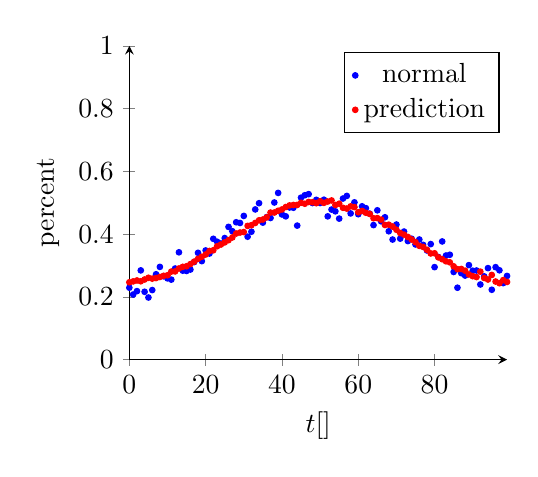
\begin{tikzpicture}
	\begin{axis}[
		xlabel={$t [\SI{}{\second}]$},
		ylabel=percent,
		axis x line=bottom,
		axis y line=left,
		ymin=0,
		ymax=1,
		scale=0.7
]
	\addplot[only marks, mark size=1pt, color=blue, mark=*] plot coordinates {
(0, 0.22927856)
(1, 0.2074585)
(2, 0.21832275)
(3, 0.2843933)
(4, 0.21618652)
(5, 0.19799805)
(6, 0.22167969)
(7, 0.2720642)
(8, 0.29553223)
(9, 0.26553345)
(10, 0.25897217)
(11, 0.25497437)
(12, 0.29037476)
(13, 0.34197998)
(14, 0.28347778)
(15, 0.2826233)
(16, 0.28707886)
(17, 0.3109436)
(18, 0.34033203)
(19, 0.3139038)
(20, 0.3479004)
(21, 0.33807373)
(22, 0.38504028)
(23, 0.3756714)
(24, 0.37008667)
(25, 0.38729858)
(26, 0.42303467)
(27, 0.40914917)
(28, 0.43780518)
(29, 0.43545532)
(30, 0.45791626)
(31, 0.39175415)
(32, 0.4076233)
(33, 0.4786682)
(34, 0.49853516)
(35, 0.43655396)
(36, 0.45401)
(37, 0.45135498)
(38, 0.5007324)
(39, 0.5312805)
(40, 0.46258545)
(41, 0.45663452)
(42, 0.48486328)
(43, 0.4840088)
(44, 0.4270935)
(45, 0.5161133)
(46, 0.52386475)
(47, 0.52737427)
(48, 0.499115)
(49, 0.50912476)
(50, 0.49905396)
(51, 0.5095825)
(52, 0.456604)
(53, 0.47817993)
(54, 0.47262573)
(55, 0.44943237)
(56, 0.5133362)
(57, 0.52163696)
(58, 0.46591187)
(59, 0.50115967)
(60, 0.4633484)
(61, 0.4885559)
(62, 0.48269653)
(63, 0.46520996)
(64, 0.42874146)
(65, 0.47583008)
(66, 0.44067383)
(67, 0.45367432)
(68, 0.40908813)
(69, 0.3826599)
(70, 0.43048096)
(71, 0.38565063)
(72, 0.40811157)
(73, 0.37771606)
(74, 0.38519287)
(75, 0.36706543)
(76, 0.3828125)
(77, 0.36572266)
(78, 0.34799194)
(79, 0.36816406)
(80, 0.2947693)
(81, 0.32702637)
(82, 0.37664795)
(83, 0.33169556)
(84, 0.33422852)
(85, 0.27938843)
(86, 0.22918701)
(87, 0.27545166)
(88, 0.26791382)
(89, 0.30114746)
(90, 0.28326416)
(91, 0.28396606)
(92, 0.23947144)
(93, 0.26531982)
(94, 0.29159546)
(95, 0.22265625)
(96, 0.29467773)
(97, 0.284729)
(98, 0.24380493)
(99, 0.2666626)
	};
	\addplot[only marks, mark size=1pt, color=red, mark=*] plot coordinates {
(0, 0.24646309)
(1, 0.24927223)
(2, 0.2523098)
(3, 0.24973524)
(4, 0.25533468)
(5, 0.2608363)
(6, 0.2580883)
(7, 0.2600216)
(8, 0.2633434)
(9, 0.2671721)
(10, 0.26879904)
(11, 0.28058052)
(12, 0.2811275)
(13, 0.29049402)
(14, 0.29562676)
(15, 0.29751024)
(16, 0.3044065)
(17, 0.31228256)
(18, 0.3212965)
(19, 0.32784778)
(20, 0.3349321)
(21, 0.34619692)
(22, 0.34842777)
(23, 0.36124367)
(24, 0.3667848)
(25, 0.37360936)
(26, 0.38073543)
(27, 0.38936585)
(28, 0.40183386)
(29, 0.40504545)
(30, 0.40648168)
(31, 0.4262132)
(32, 0.4283422)
(33, 0.43562445)
(34, 0.44393831)
(35, 0.44649827)
(36, 0.45345068)
(37, 0.46858084)
(38, 0.46877068)
(39, 0.4743431)
(40, 0.4785128)
(41, 0.48623627)
(42, 0.49152142)
(43, 0.49279627)
(44, 0.49301612)
(45, 0.4997137)
(46, 0.49672985)
(47, 0.50240564)
(48, 0.5015566)
(49, 0.49861723)
(50, 0.50468385)
(51, 0.49952948)
(52, 0.5038705)
(53, 0.5072257)
(54, 0.49271286)
(55, 0.49685216)
(56, 0.48378494)
(57, 0.48133856)
(58, 0.4884061)
(59, 0.48600978)
(60, 0.46958733)
(61, 0.47389764)
(62, 0.4679124)
(63, 0.46436)
(64, 0.45063794)
(65, 0.45094436)
(66, 0.44617844)
(67, 0.42914882)
(68, 0.4300288)
(69, 0.42413294)
(70, 0.41397488)
(71, 0.403247)
(72, 0.39835995)
(73, 0.39095232)
(74, 0.38294864)
(75, 0.37433046)
(76, 0.36259735)
(77, 0.3591426)
(78, 0.35018468)
(79, 0.338364)
(80, 0.33886778)
(81, 0.32589227)
(82, 0.31995645)
(83, 0.31323838)
(84, 0.3100605)
(85, 0.29732224)
(86, 0.2883816)
(87, 0.28898352)
(88, 0.28356954)
(89, 0.27142316)
(90, 0.26598096)
(91, 0.26319492)
(92, 0.280414)
(93, 0.26025814)
(94, 0.2553401)
(95, 0.26981425)
(96, 0.2488755)
(97, 0.24358332)
(98, 0.25348443)
(99, 0.2476387)
	};
	\addlegendentry{normal}
	\addlegendentry{prediction}
	\end{axis}
\end{tikzpicture}

	\end{minipage}
	\begin{minipage}[t]{0.45\textwidth}
			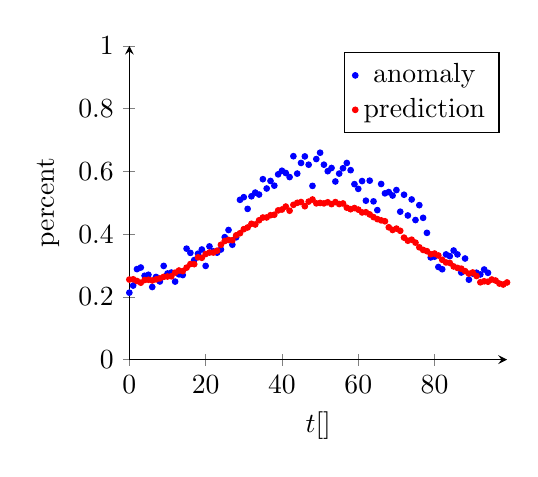
\begin{tikzpicture}
	\begin{axis}[
		xlabel={$t [\SI{}{\second}]$},
		ylabel=percent,
		axis x line=bottom,
		axis y line=left,
		ymin=0,
		ymax=1,
		scale=0.7
]
	\addplot[only marks, mark size=1pt, color=blue, mark=*] plot coordinates {
(0, 0.2133789)
(1, 0.23602295)
(2, 0.28845215)
(3, 0.29354858)
(4, 0.26727295)
(5, 0.27035522)
(6, 0.23147583)
(7, 0.26345825)
(8, 0.24908447)
(9, 0.2986145)
(10, 0.27450562)
(11, 0.27752686)
(12, 0.24874878)
(13, 0.271698)
(14, 0.26953125)
(15, 0.35369873)
(16, 0.34017944)
(17, 0.31723022)
(18, 0.33761597)
(19, 0.35092163)
(20, 0.29864502)
(21, 0.36080933)
(22, 0.3451538)
(23, 0.34088135)
(24, 0.35095215)
(25, 0.3902893)
(26, 0.41308594)
(27, 0.36624146)
(28, 0.38986206)
(29, 0.5091858)
(30, 0.5176697)
(31, 0.4803772)
(32, 0.5204468)
(33, 0.5322876)
(34, 0.5260315)
(35, 0.5749817)
(36, 0.5453491)
(37, 0.569397)
(38, 0.55441284)
(39, 0.5904236)
(40, 0.6018677)
(41, 0.59472656)
(42, 0.5817566)
(43, 0.6482544)
(44, 0.59280396)
(45, 0.62677)
(46, 0.6475525)
(47, 0.6211853)
(48, 0.55371094)
(49, 0.6391907)
(50, 0.6593628)
(51, 0.62124634)
(52, 0.6005249)
(53, 0.6107178)
(54, 0.5676575)
(55, 0.5928345)
(56, 0.6099243)
(57, 0.62667847)
(58, 0.60369873)
(59, 0.5592041)
(60, 0.5441284)
(61, 0.56900024)
(62, 0.5064697)
(63, 0.570343)
(64, 0.504303)
(65, 0.4764099)
(66, 0.5596924)
(67, 0.5298767)
(68, 0.53393555)
(69, 0.5228882)
(70, 0.54034424)
(71, 0.47140503)
(72, 0.5254822)
(73, 0.45941162)
(74, 0.510376)
(75, 0.44485474)
(76, 0.49224854)
(77, 0.45181274)
(78, 0.40402222)
(79, 0.32565308)
(80, 0.328125)
(81, 0.29519653)
(82, 0.2880249)
(83, 0.33529663)
(84, 0.32989502)
(85, 0.3477478)
(86, 0.33529663)
(87, 0.27755737)
(88, 0.32229614)
(89, 0.25476074)
(90, 0.27438354)
(91, 0.276886)
(92, 0.27145386)
(93, 0.2871704)
(94, 0.2765808)
	};
	\addplot[only marks, mark size=1pt, color=red, mark=*] plot coordinates {

(0, 0.25517547)
(1, 0.25596672)
(2, 0.2505421)
(3, 0.2451446)
(4, 0.2536649)
(5, 0.25459528)
(6, 0.2523541)
(7, 0.25567627)
(8, 0.25897074)
(9, 0.26382625)
(10, 0.2649119)
(11, 0.2655142)
(12, 0.2772423)
(13, 0.28393567)
(14, 0.2820531)
(15, 0.29314294)
(16, 0.30453762)
(17, 0.30425388)
(18, 0.32606268)
(19, 0.32451057)
(20, 0.33647186)
(21, 0.34116146)
(22, 0.34121227)
(23, 0.34719998)
(24, 0.3659501)
(25, 0.3779876)
(26, 0.3813619)
(27, 0.38061115)
(28, 0.39612374)
(29, 0.40282616)
(30, 0.41570908)
(31, 0.4210897)
(32, 0.4328343)
(33, 0.4306392)
(34, 0.44401854)
(35, 0.45284593)
(36, 0.4530311)
(37, 0.46016362)
(38, 0.4617548)
(39, 0.4754996)
(40, 0.47832155)
(41, 0.4877711)
(42, 0.47457412)
(43, 0.4932733)
(44, 0.49966103)
(45, 0.502202)
(46, 0.4888865)
(47, 0.5035607)
(48, 0.51031786)
(49, 0.4980901)
(50, 0.4994049)
(51, 0.49790707)
(52, 0.50142944)
(53, 0.4955338)
(54, 0.5020641)
(55, 0.4958108)
(56, 0.4976046)
(57, 0.48410338)
(58, 0.47938585)
(59, 0.48302588)
(60, 0.4780665)
(61, 0.4690646)
(62, 0.46973258)
(63, 0.46270987)
(64, 0.4541604)
(65, 0.44783998)
(66, 0.44379902)
(67, 0.44097963)
(68, 0.4217441)
(69, 0.41320667)
(70, 0.41754586)
(71, 0.41051432)
(72, 0.38880774)
(73, 0.37895176)
(74, 0.3821065)
(75, 0.37280777)
(76, 0.35792762)
(77, 0.34956065)
(78, 0.34564692)
(79, 0.33592197)
(80, 0.33804682)
(81, 0.33185786)
(82, 0.3180303)
(83, 0.30977106)
(84, 0.3081681)
(85, 0.29693812)
(86, 0.29236597)
(87, 0.28984982)
(88, 0.28199905)
(89, 0.27408743)
(90, 0.27773026)
(91, 0.26656723)
(92, 0.2464428)
(93, 0.24968585)
(94, 0.24833006)
(95, 0.25528675)
(96, 0.25201452)
(97, 0.2423881)
(98, 0.23940933)
(99, 0.24589372)
	};
	\addlegendentry{anomaly}
	\addlegendentry{prediction}
	\end{axis}
\end{tikzpicture}

	\end{minipage}
	\caption{Input and output of the \ac{aec} with normal and anomalous data.}
	\label{f:aec_deep}
	\end{figure}

	\subsection{Support Vector Machine}
	In the case of \acp{svm}, a special change had to be made for the training. As \acp{svm} are only available as trainable kernel machines \cite{tf-svm} in tensorflow, labels had to be added to the training set. But in general it has been shown that \acp{svm} can also be successfully trained unsupervised, as so called One-Class SVM \cite{one-class-svm}.
	
	To train the network, a rather high number of epochs has to be used. After around 10 epochs the \ac{svm} stopped converging, unfortunately with a still quite high prediction error. But as the model uses only the \ac{svm} layer, which is mapped to an output layer of two variables, this uncertainty might be reasonable. The two output variables are referring to anomaly ($y_+$) and non-anomaly ($y_-$). \newline
	The used layer dimension with 2048 nodes was also quite high to achieve a reasonable accuracy. As a result, the computation to train the neural network got substantially bigger than the \ac{aec}.
		
	To now separate normal and anomalous datasets after the training, the two variables ($y_+$ and $y_-$) on the output were compared. Whichever had the higher result made the decision for normal and anomalous. This did yield the lowest false-positive rate with 0.0\%. But this also had rather low true-positive rate being much below 50\%. \newline
	To further increase the true-positive rate the boundary decisions were shifted. This was done by averaging the predictions $y_+$ and $y_-$ for the training set and shifting these values towards to the edge of their miss-categorization. In the following an example calculation for the corrected anomaly output $\hat{y}_+$ is given:
	
	\begin{align*}
	\overline{y}_{pp} &= \frac{1}{N_+}\cdot \sum_{i=1}^N y_+ (\mathbf{x}_i) \cdot \alpha_i \\
	\overline{y}_{fp} &= \frac{1}{N_-}\cdot \sum_{i=1}^N y_+ (\mathbf{x}_i) \cdot \left| \alpha_i - 1 \right| \\
	\hat{y}_+ &= \frac{\overline{y}_{pp} - \overline{y}_{fp}}{10} + \overline{y}_{fp}
	\end{align*}

	Here $\alpha_i$ equals one for anomalies and zero for normal data. To put the equation into words, the average miss-categorization level (false-positive) of the anomaly output $y_+$ is shifted 10\% towards its way to the average true-positive level. Therefore every $y_+(\mathbf{x})$ value above $\hat{y}_+$ is counted as anomalous. The same procedure is applied to the normal output $y_-(\mathbf{x})$.
	
	In conclusion, a \ac{svm} might not be a good solution to analyse these kind of datasets with high noise and rather subtle differences between normal and anomalous examples.
	
	\subsection{Long-Short-term Memory}
	As \acp{lstm} are used for predictions, the use of the datasets is getting slightly modified. To learn a future prediction from a given set, the network is given an input of $\mathbf{x}_i$ and should predict an output of $\mathbf{x}_{i+1}$ for the following orbit. Hence the input and output datasets were still from the same dataset, but shifted by one orbit. \newline
	The prediction time here doesn't need to be necessarily one orbit period. For example, one could also chose a sliding window and only predict a few minutes ahead. Here we chose to just always predict the following orbit from a previous one. Thus the \ac{lstm} only needs one cell layer. 

	The cut-off value was chosen the same way as it was done with the \ac{aec}. To now take a look on what the predictions of the \ac{lstm} are for the normal and anomalous data, the graphs in figure \ref{f:lstm_deep} are given. On the left the normal curve is shown and on the right the anomalous one. Again, just like the \ac{aec} the \ac{lstm} learned a normal presentation of the data as the anomalies in the training data occurred randomly. \newline
	Unfortunately this example can't show the true potential of \acp{lstm}. An \ac{lstm} could learn for example multiple patterns as well as their sequence if they are periodical.
		
	\begin{figure}[htb]
	\centering
	\begin{minipage}[t]{0.45\textwidth}
			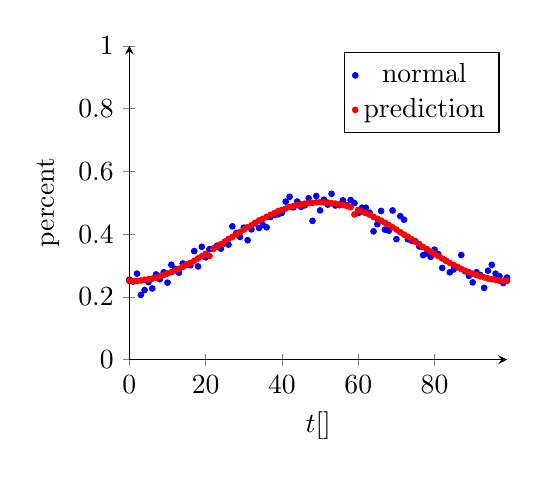
\begin{tikzpicture}
	\begin{axis}[
		xlabel={$t [\SI{}{\second}]$},
		ylabel=percent,
		axis x line=bottom,
		axis y line=left,
		ymin=0,
		ymax=1,
		scale=0.7
]
	\addplot[only marks, mark size=1pt, color=blue, mark=*] plot coordinates {
(0, 0.25494385)
(1, 0.24847412)
(2, 0.27401733)
(3, 0.20605469)
(4, 0.2218628)
(5, 0.24716187)
(6, 0.22698975)
(7, 0.27157593)
(8, 0.25628662)
(9, 0.27838135)
(10, 0.24539185)
(11, 0.3022766)
(12, 0.28918457)
(13, 0.2770691)
(14, 0.30633545)
(15, 0.3026123)
(16, 0.3007202)
(17, 0.3458557)
(18, 0.29708862)
(19, 0.35964966)
(20, 0.32595825)
(21, 0.35198975)
(22, 0.354187)
(23, 0.36315918)
(24, 0.3536682)
(25, 0.37039185)
(26, 0.36657715)
(27, 0.42471313)
(28, 0.40307617)
(29, 0.39102173)
(30, 0.42053223)
(31, 0.38061523)
(32, 0.41513062)
(33, 0.43432617)
(34, 0.41952515)
(35, 0.42889404)
(36, 0.42156982)
(37, 0.45458984)
(38, 0.46099854)
(39, 0.4628601)
(40, 0.46780396)
(41, 0.50341797)
(42, 0.5189209)
(43, 0.48535156)
(44, 0.50390625)
(45, 0.4869995)
(46, 0.4916687)
(47, 0.5141907)
(48, 0.4421997)
(49, 0.52142334)
(50, 0.47555542)
(51, 0.5095215)
(52, 0.49404907)
(53, 0.5285034)
(54, 0.4911499)
(55, 0.49206543)
(56, 0.50775146)
(57, 0.49221802)
(58, 0.50857544)
(59, 0.4987793)
(60, 0.46713257)
(61, 0.48410034)
(62, 0.48391724)
(63, 0.46798706)
(64, 0.40878296)
(65, 0.4316101)
(66, 0.47384644)
(67, 0.41427612)
(68, 0.41085815)
(69, 0.47540283)
(70, 0.3840027)
(71, 0.457489)
(72, 0.44589233)
(73, 0.38342285)
(74, 0.3791809)
(75, 0.3770752)
(76, 0.36047363)
(77, 0.33303833)
(78, 0.3385315)
(79, 0.3274536)
(80, 0.35025024)
(81, 0.3360901)
(82, 0.29241943)
(83, 0.31524658)
(84, 0.2782898)
(85, 0.28753662)
(86, 0.29440308)
(87, 0.3333435)
(88, 0.28128052)
(89, 0.26690674)
(90, 0.2461853)
(91, 0.2784729)
(92, 0.26971436)
(93, 0.22866821)
(94, 0.28329468)
(95, 0.30203247)
(96, 0.27383423)
(97, 0.26593018)
(98, 0.24423218)
(99, 0.26153564)
};
	\addplot[only marks, mark size=1pt, color=red, mark=*] plot coordinates {
(0, 0.25057802)
(1, 0.250705)
(2, 0.250706)
(3, 0.25215992)
(4, 0.2544506)
(5, 0.2557756)
(6, 0.25819093)
(7, 0.26157653)
(8, 0.26559252)
(9, 0.2698741)
(10, 0.27431747)
(11, 0.27846593)
(12, 0.28399077)
(13, 0.28944853)
(14, 0.29575258)
(15, 0.30197245)
(16, 0.30812874)
(17, 0.3150881)
(18, 0.32241306)
(19, 0.3294862)
(20, 0.3371979)
(21, 0.33020195)
(22, 0.35229906)
(23, 0.35930648)
(24, 0.36800903)
(25, 0.37606233)
(26, 0.3846135)
(27, 0.39104015)
(28, 0.39887297)
(29, 0.40663475)
(30, 0.4142397)
(31, 0.42206788)
(32, 0.427763)
(33, 0.436069)
(34, 0.44359726)
(35, 0.4487256)
(36, 0.4551902)
(37, 0.46126273)
(38, 0.46664184)
(39, 0.4733037)
(40, 0.4770921)
(41, 0.48130438)
(42, 0.4865906)
(43, 0.48934552)
(44, 0.49248984)
(45, 0.49469894)
(46, 0.496839)
(47, 0.49890214)
(48, 0.49955946)
(49, 0.50088936)
(50, 0.50186753)
(51, 0.50136197)
(52, 0.5006228)
(53, 0.4985591)
(54, 0.49720418)
(55, 0.49458212)
(56, 0.49295056)
(57, 0.48950833)
(58, 0.4858226)
(59, 0.46280798)
(60, 0.47697118)
(61, 0.47171405)
(62, 0.46669617)
(63, 0.4619239)
(64, 0.45495936)
(65, 0.4489432)
(66, 0.4429253)
(67, 0.43605188)
(68, 0.42923442)
(69, 0.42185876)
(70, 0.41435957)
(71, 0.40622824)
(72, 0.39837065)
(73, 0.39145678)
(74, 0.38354126)
(75, 0.3756699)
(76, 0.3679754)
(77, 0.3586755)
(78, 0.35210696)
(79, 0.3444079)
(80, 0.33654067)
(81, 0.3297064)
(82, 0.32247913)
(83, 0.31506267)
(84, 0.3079031)
(85, 0.30143642)
(86, 0.2955792)
(87, 0.28878582)
(88, 0.2835553)
(89, 0.27893913)
(90, 0.27383637)
(91, 0.26953533)
(92, 0.26540434)
(93, 0.2620207)
(94, 0.25871044)
(95, 0.25619432)
(96, 0.2542893)
(97, 0.25153902)
(98, 0.25149256)
(99, 0.2507174)
};
	\addlegendentry{normal}
	\addlegendentry{prediction}
	\end{axis}
\end{tikzpicture}

	\end{minipage}
	\begin{minipage}[t]{0.45\textwidth}
			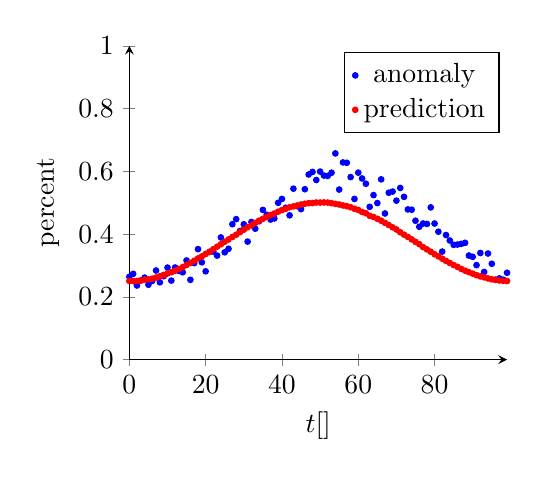
\begin{tikzpicture}
	\begin{axis}[
		xlabel={$t [\SI{}{\second}]$},
		ylabel=percent,
		axis x line=bottom,
		axis y line=left,
		ymin=0,
		ymax=1,
		scale=0.7
]
	\addplot[only marks, mark size=1pt, color=blue, mark=*] plot coordinates {
(0, 0.2642212)
(1, 0.27337646)
(2, 0.23623657)
(3, 0.2522583)
(4, 0.26138306)
(5, 0.23864746)
(6, 0.2510376)
(7, 0.28396606)
(8, 0.24630737)
(9, 0.26583862)
(10, 0.2932434)
(11, 0.25183105)
(12, 0.29351807)
(13, 0.28271484)
(14, 0.2782898)
(15, 0.31607056)
(16, 0.25424194)
(17, 0.3074646)
(18, 0.35214233)
(19, 0.3100586)
(20, 0.2814331)
(21, 0.34347534)
(22, 0.34436035)
(23, 0.33148193)
(24, 0.3894043)
(25, 0.34194946)
(26, 0.35317993)
(27, 0.43164062)
(28, 0.44763184)
(29, 0.4102173)
(30, 0.43130493)
(31, 0.37612915)
(32, 0.43859863)
(33, 0.41723633)
(34, 0.440979)
(35, 0.47717285)
(36, 0.46170044)
(37, 0.44638062)
(38, 0.4498291)
(39, 0.49972534)
(40, 0.5121155)
(41, 0.48388672)
(42, 0.45986938)
(43, 0.5448303)
(44, 0.4890442)
(45, 0.4794922)
(46, 0.5430298)
(47, 0.5899048)
(48, 0.59814453)
(49, 0.5724182)
(50, 0.59921265)
(51, 0.58651733)
(52, 0.58551025)
(53, 0.5956116)
(54, 0.6571655)
(55, 0.54193115)
(56, 0.62841797)
(57, 0.6272583)
(58, 0.58169556)
(59, 0.5120239)
(60, 0.5958252)
(61, 0.57736206)
(62, 0.5605774)
(63, 0.48687744)
(64, 0.524292)
(65, 0.49893188)
(66, 0.5744629)
(67, 0.46575928)
(68, 0.53182983)
(69, 0.535553)
(70, 0.50668335)
(71, 0.54711914)
(72, 0.5187073)
(73, 0.47869873)
(74, 0.47769165)
(75, 0.4425354)
(76, 0.4234314)
(77, 0.43371582)
(78, 0.4324646)
(79, 0.48510742)
(80, 0.43371582)
(81, 0.4076233)
(82, 0.34429932)
(83, 0.39709473)
(84, 0.37963867)
(85, 0.3657837)
(86, 0.36676025)
(87, 0.36889648)
(88, 0.3722229)
(89, 0.33166504)
(90, 0.32757568)
(91, 0.3010559)
(92, 0.3399048)
(93, 0.2793274)
(94, 0.33813477)
(95, 0.30551147)
(96, 0.25497437)
(97, 0.25881958)
(98, 0.25457764)
(99, 0.27679443)
};
	\addplot[only marks, mark size=1pt, color=red, mark=*] plot coordinates {
(0, 0.25057492)
(1, 0.25007093)
(2, 0.2508472)
(3, 0.25182036)
(4, 0.2548628)
(5, 0.2557395)
(6, 0.25806084)
(7, 0.26159734)
(8, 0.26574045)
(9, 0.26983982)
(10, 0.27443653)
(11, 0.27848184)
(12, 0.28341177)
(13, 0.28870478)
(14, 0.29487184)
(15, 0.30188575)
(16, 0.30808866)
(17, 0.31505203)
(18, 0.3225799)
(19, 0.3288647)
(20, 0.33677748)
(21, 0.3431157)
(22, 0.35192984)
(23, 0.35984555)
(24, 0.36763617)
(25, 0.37557608)
(26, 0.38294038)
(27, 0.39081457)
(28, 0.3980862)
(29, 0.40636337)
(30, 0.41422445)
(31, 0.42196617)
(32, 0.42774197)
(33, 0.4357839)
(34, 0.44287187)
(35, 0.44860154)
(36, 0.45464125)
(37, 0.460778)
(38, 0.46546984)
(39, 0.47145668)
(40, 0.47661516)
(41, 0.48066464)
(42, 0.48552188)
(43, 0.48834744)
(44, 0.49122992)
(45, 0.49421832)
(46, 0.49667996)
(47, 0.49860853)
(48, 0.49903664)
(49, 0.500661)
(50, 0.5005096)
(51, 0.50094557)
(52, 0.500507)
(53, 0.49849027)
(54, 0.49632865)
(55, 0.49433634)
(56, 0.49128437)
(57, 0.4890678)
(58, 0.4856617)
(59, 0.48069733)
(60, 0.47695422)
(61, 0.47041062)
(62, 0.46664733)
(63, 0.4583739)
(64, 0.45464987)
(65, 0.44878238)
(66, 0.44278967)
(67, 0.43582442)
(68, 0.42878145)
(69, 0.4215377)
(70, 0.414792)
(71, 0.40590477)
(72, 0.3982379)
(73, 0.39110464)
(74, 0.38337138)
(75, 0.37529832)
(76, 0.36793265)
(77, 0.3584491)
(78, 0.3513085)
(79, 0.34387198)
(80, 0.33584863)
(81, 0.3292976)
(82, 0.32167086)
(83, 0.31467712)
(84, 0.30787152)
(85, 0.30142722)
(86, 0.2957924)
(87, 0.28895685)
(88, 0.2835246)
(89, 0.27881148)
(90, 0.27397856)
(91, 0.26924708)
(92, 0.265195)
(93, 0.2621557)
(94, 0.25879058)
(95, 0.25598806)
(96, 0.25412446)
(97, 0.2521264)
(98, 0.2511632)
(99, 0.25062808)
};
	\addlegendentry{anomaly}
	\addlegendentry{prediction}
	\end{axis}
\end{tikzpicture}

	\end{minipage}
	\caption{Input and future prediction of the \ac{lstm} with normal and anomalous data}
	\label{f:lstm_deep}
	\end{figure}	
	
	\subsection{Test Results and Comparison}
	For comparison the 	true-positive rates of the three detection techniques are analysed. Additionally the false-positive rate is shown to check for any irregularities. 

	The graphs of the results are shown in the following chapters, see figure \ref{f:slope}, \ref{f:pulse} and \ref{f:sine}. Generally speaking, there are no huge differences between the detection techniques. Only the \ac{svm} seems to have a slight disadvantage in the overall comparison, especially in the domain of sine anomalies. The \ac{aec} and \ac{lstm} perform almost equally well. \newline %TODO signal-to-noise-ratio
	If one takes a look at the absolute numbers where the detection reaches almost a hundred percent, it can be noticed that the difference between normal and anomalous data are quite small and almost indistinguishable for a human. To illustrate this, the example of the pulse anomaly is taken. Here the detection is already at 100\% at the height $h=1.1$. Speaking of current sensors, an increase of 10\% in the current would lead to a power increase 21\% above normal, which is usually well below the critical limit.
	
	In the following the test results are discussed in more detail.	
	
	\subsubsection{Slope Anomaly}
	The slope anomaly results are presented in figure \ref{f:slope}. The anomaly was detected by all techniques equally. This implies also, that a drifting sensor might be detected in an early, non-critical state. \newline
	The detection of 100\% is met at a slope of $m \approx \num{2.5e-3}$, which is equivalent to a total value increase of $\approx 12\%$ over the course of 50 minutes.
	
\begin{figure}[htb]
\centering
\begin{minipage}[t]{0.45\textwidth}
		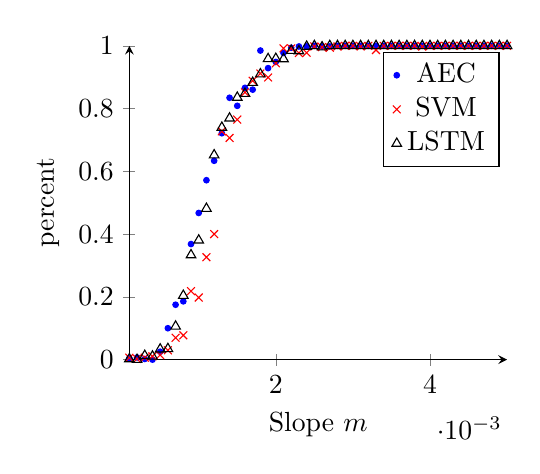
\begin{tikzpicture}
	\begin{axis}[
		xlabel={Slope $m$},
		ylabel={percent},
		axis x line=bottom,
		axis y line=left,
		ymin=0,
		ymax=1,
scale=0.7
]
	\addplot[only marks, mark size=1pt, color=blue, mark=*] plot coordinates {
		(0.0001, 0.004106776180698)
		(0.0002, 0.006960556844548)
		(0.0003, 0.002087682672234)
		(0.0004, 0.0)
		(0.0005, 0.025210084033614)
		(0.0006, 0.100080191122175)
		(0.0007, 0.174950298210736)
		(0.0008, 0.185714285714286)
		(0.0009, 0.368312757201646)
		(0.001, 0.467368421052632)
		(0.0011, 0.571725571725572)
		(0.0012, 0.633684210526316)
		(0.0013, 0.721442885771543)
		(0.0014, 0.834437086092715)
		(0.0015, 0.808743169398907)
		(0.0016, 0.866108786610879)
		(0.0017, 0.860262008733625)
		(0.0018, 0.984913793103448)
		(0.0019, 0.928853754940711)
		(0.002, 0.948559670781893)
		(0.0021, 0.977319587628866)
		(0.0022, 0.993839835728953)
		(0.0023, 0.997920997920998)
		(0.0024, 0.998003992015968)
		(0.0025, 1.0)
		(0.0026, 0.997916666666667)
		(0.0027, 0.997983870967742)
		(0.0028, 1.0)
		(0.0029, 1.0)
		(0.003, 1.0)
		(0.0031, 1.0)
		(0.0032, 1.0)
		(0.0033, 1.0)
		(0.0034, 1.0)
		(0.0035, 1.0)
		(0.0036, 1.0)
		(0.0037, 1.0)
		(0.0038, 1.0)
		(0.0039, 1.0)
		(0.004, 1.0)
		(0.0041, 1.0)
		(0.0042, 1.0)
		(0.0043, 1.0)
		(0.0044, 1.0)
		(0.0045, 1.0)
		(0.0046, 1.0)
		(0.0047, 1.0)
		(0.0048, 1.0)
		(0.0049, 1.0)
		(0.005, 1.0)
	};
	\addlegendentry{AEC}
	\addplot[only marks, color=red, mark=x] plot coordinates {
		(0.0001, 0.006160164271047)
		(0.0002, 0.002320185614849)
		(0.0003, 0.006263048016701)
		(0.0004, 0.010683760683761)
		(0.0005, 0.014705882352941)
		(0.0006, 0.029723991507431)
		(0.0007, 0.069582504970179)
		(0.0008, 0.077551020408163)
		(0.0009, 0.218106995884774)
		(0.001, 0.197894736842105)
		(0.0011, 0.326403326403326)
		(0.0012, 0.4)
		(0.0013, 0.727454909819639)
		(0.0014, 0.706401766004415)
		(0.0015, 0.765027322404372)
		(0.0016, 0.851464435146444)
		(0.0017, 0.888646288209607)
		(0.0018, 0.911637931034483)
		(0.0019, 0.899209486166008)
		(0.002, 0.944444444444444)
		(0.0021, 0.991752577319588)
		(0.0022, 0.991786447638604)
		(0.0023, 0.977130977130977)
		(0.0024, 0.978043912175649)
		(0.0025, 0.997912317327766)
		(0.0026, 0.995833333333333)
		(0.0027, 0.993951612903226)
		(0.0028, 0.997894736842105)
		(0.0029, 1.0)
		(0.003, 1.0)
		(0.0031, 0.997955010224949)
		(0.0032, 1.0)
		(0.0033, 0.986636971046771)
		(0.0034, 1.0)
		(0.0035, 1.0)
		(0.0036, 1.0)
		(0.0037, 1.0)
		(0.0038, 1.0)
		(0.0039, 0.997701149425287)
		(0.004, 1.0)
		(0.0041, 1.0)
		(0.0042, 1.0)
		(0.0043, 1.0)
		(0.0044, 1.0)
		(0.0045, 1.0)
		(0.0046, 1.0)
		(0.0047, 1.0)
		(0.0048, 1.0)
		(0.0049, 1.0)
		(0.005, 1.0)
	};
	\addlegendentry{SVM}
	\addplot[only marks, color=black, mark=triangle] plot coordinates {
		(0.0001, 0.002016129032258)
		(0.0002, 0.0)
		(0.0003, 0.01271186440678)
		(0.0004, 0.010615711252654)
		(0.0005, 0.033259423503326)
		(0.0006, 0.034557235421166)
		(0.0007, 0.106060606060606)
		(0.0008, 0.204123711340206)
		(0.0009, 0.333333333333333)
		(0.001, 0.38034188034188)
		(0.0011, 0.481335952848723)
		(0.0012, 0.651804670912951)
		(0.0013, 0.739696312364425)
		(0.0014, 0.769067796610169)
		(0.0015, 0.835416666666667)
		(0.0016, 0.847826086956522)
		(0.0017, 0.882716049382716)
		(0.0018, 0.91002044989775)
		(0.0019, 0.958419958419958)
		(0.002, 0.959139784946236)
		(0.0021, 0.958071278825996)
		(0.0022, 0.984848484848485)
		(0.0023, 0.983402489626556)
		(0.0024, 0.997899159663866)
		(0.0025, 1.0)
		(0.0026, 0.995841995841996)
		(0.0027, 1.0)
		(0.0028, 1.0)
		(0.0029, 1.0)
		(0.003, 1.0)
		(0.0031, 1.0)
		(0.0032, 1.0)
		(0.0033, 1.0)
		(0.0034, 1.0)
		(0.0035, 1.0)
		(0.0036, 1.0)
		(0.0037, 1.0)
		(0.0038, 1.0)
		(0.0039, 1.0)
		(0.004, 1.0)
		(0.0041, 1.0)
		(0.0042, 1.0)
		(0.0043, 1.0)
		(0.0044, 1.0)
		(0.0045, 1.0)
		(0.0046, 1.0)
		(0.0047, 1.0)
		(0.0048, 1.0)
		(0.0049, 1.0)
		(0.005, 1.0)
	};
	\addlegendentry{LSTM}
	\end{axis}
\end{tikzpicture}

		\subcaption{True-Positive rate}
\end{minipage}
\begin{minipage}[t]{0.45\textwidth}
		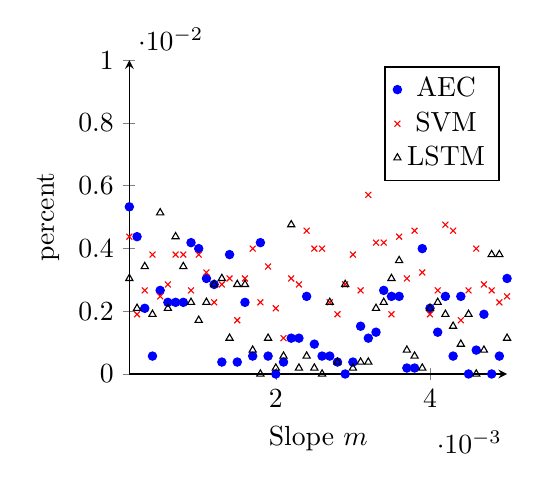
\begin{tikzpicture}
	\begin{axis}[
		xlabel={Slope $m$},
		ylabel={percent},
		axis x line=bottom,
		axis y line=left,
		ymin=0,
		ymax=0.01,
scale=0.7
]
	\addplot[only marks, mark size=1.5, color=blue, mark=*] plot coordinates {
		(0.0001, 0.005327245053272)
		(0.0002, 0.00437595129376)
		(0.0003, 0.002092846270928)
		(0.0004, 0.000570776255708)
		(0.0005, 0.002663622526636)
		(0.0006, 0.002283105022831)
		(0.0007, 0.002283105022831)
		(0.0008, 0.002283105022831)
		(0.0009, 0.004185692541857)
		(0.001, 0.003995433789954)
		(0.0011, 0.003044140030441)
		(0.0012, 0.002853881278539)
		(0.0013, 0.000380517503805)
		(0.0014, 0.003805175038052)
		(0.0015, 0.000380517503805)
		(0.0016, 0.002283105022831)
		(0.0017, 0.000570776255708)
		(0.0018, 0.004185692541857)
		(0.0019, 0.000570776255708)
		(0.002, 0.0)
		(0.0021, 0.000380517503805)
		(0.0022, 0.001141552511416)
		(0.0023, 0.001141552511416)
		(0.0024, 0.002473363774734)
		(0.0025, 0.000951293759513)
		(0.0026, 0.000570776255708)
		(0.0027, 0.000570776255708)
		(0.0028, 0.000380517503805)
		(0.0029, 0.0)
		(0.003, 0.000380517503805)
		(0.0031, 0.001522070015221)
		(0.0032, 0.001141552511416)
		(0.0033, 0.001331811263318)
		(0.0034, 0.002663622526636)
		(0.0035, 0.002473363774734)
		(0.0036, 0.002473363774734)
		(0.0037, 0.000190258751903)
		(0.0038, 0.000190258751903)
		(0.0039, 0.003995433789954)
		(0.004, 0.002092846270928)
		(0.0041, 0.001331811263318)
		(0.0042, 0.002473363774734)
		(0.0043, 0.000570776255708)
		(0.0044, 0.002473363774734)
		(0.0045, 0.0)
		(0.0046, 0.00076103500761)
		(0.0047, 0.001902587519026)
		(0.0048, 0.0)
		(0.0049, 0.000570776255708)
		(0.005, 0.003044140030441)
	};
	\addlegendentry{AEC}
	\addplot[only marks, mark size=1.5, color=red, mark=x] plot coordinates {
		(0.0001, 0.00437595129376)
		(0.0002, 0.001902587519026)
		(0.0003, 0.002663622526636)
		(0.0004, 0.003805175038052)
		(0.0005, 0.002473363774734)
		(0.0006, 0.002853881278539)
		(0.0007, 0.003805175038052)
		(0.0008, 0.003805175038052)
		(0.0009, 0.002663622526636)
		(0.001, 0.003805175038052)
		(0.0011, 0.003234398782344)
		(0.0012, 0.002283105022831)
		(0.0013, 0.002853881278539)
		(0.0014, 0.003044140030441)
		(0.0015, 0.001712328767123)
		(0.0016, 0.003044140030441)
		(0.0017, 0.003995433789954)
		(0.0018, 0.002283105022831)
		(0.0019, 0.003424657534247)
		(0.002, 0.002092846270928)
		(0.0021, 0.001141552511416)
		(0.0022, 0.003044140030441)
		(0.0023, 0.002853881278539)
		(0.0024, 0.004566210045662)
		(0.0025, 0.003995433789954)
		(0.0026, 0.003995433789954)
		(0.0027, 0.002283105022831)
		(0.0028, 0.001902587519026)
		(0.0029, 0.002853881278539)
		(0.003, 0.003805175038052)
		(0.0031, 0.002663622526636)
		(0.0032, 0.005707762557078)
		(0.0033, 0.004185692541857)
		(0.0034, 0.004185692541857)
		(0.0035, 0.001902587519026)
		(0.0036, 0.00437595129376)
		(0.0037, 0.003044140030441)
		(0.0038, 0.004566210045662)
		(0.0039, 0.003234398782344)
		(0.004, 0.001902587519026)
		(0.0041, 0.002663622526636)
		(0.0042, 0.004756468797565)
		(0.0043, 0.004566210045662)
		(0.0044, 0.001712328767123)
		(0.0045, 0.002663622526636)
		(0.0046, 0.003995433789954)
		(0.0047, 0.002853881278539)
		(0.0048, 0.002663622526636)
		(0.0049, 0.002283105022831)
		(0.005, 0.002473363774734)
	};
	\addlegendentry{SVM}
	\addplot[only marks, mark size=1.5, color=black, mark=triangle] plot coordinates {
		(0.0001, 0.003044719314938)
		(0.0002, 0.00209324452902)
		(0.0003, 0.003425309229305)
		(0.0004, 0.001902949571836)
		(0.0005, 0.005137963843958)
		(0.0006, 0.00209324452902)
		(0.0007, 0.004376784015224)
		(0.0008, 0.003425309229305)
		(0.0009, 0.002283539486204)
		(0.001, 0.001712654614653)
		(0.0011, 0.002283539486204)
		(0.0012, 0.002854424357755)
		(0.0013, 0.003044719314938)
		(0.0014, 0.001141769743102)
		(0.0015, 0.002854424357755)
		(0.0016, 0.002854424357755)
		(0.0017, 0.000761179828735)
		(0.0018, 0.0)
		(0.0019, 0.001141769743102)
		(0.002, 0.000190294957184)
		(0.0021, 0.000570884871551)
		(0.0022, 0.004757373929591)
		(0.0023, 0.000190294957184)
		(0.0024, 0.000570884871551)
		(0.0025, 0.000190294957184)
		(0.0026, 0.0)
		(0.0027, 0.002283539486204)
		(0.0028, 0.000380589914367)
		(0.0029, 0.002854424357755)
		(0.003, 0.000190294957184)
		(0.0031, 0.000380589914367)
		(0.0032, 0.000380589914367)
		(0.0033, 0.00209324452902)
		(0.0034, 0.002283539486204)
		(0.0035, 0.003044719314938)
		(0.0036, 0.003615604186489)
		(0.0037, 0.000761179828735)
		(0.0038, 0.000570884871551)
		(0.0039, 0.000190294957184)
		(0.004, 0.00209324452902)
		(0.0041, 0.002283539486204)
		(0.0042, 0.001902949571836)
		(0.0043, 0.001522359657469)
		(0.0044, 0.000951474785918)
		(0.0045, 0.001902949571836)
		(0.0046, 0.0)
		(0.0047, 0.000761179828735)
		(0.0048, 0.003805899143673)
		(0.0049, 0.003805899143673)
		(0.005, 0.001141769743102)
	};
	\addlegendentry{LSTM}
	\end{axis}
\end{tikzpicture}

		\subcaption{False-Positive rate}
\end{minipage}
\caption{Almost equivalent rates in the slope detection for all three techniques}
\label{f:slope}
\end{figure}
		
	\subsubsection{Pulse Anomaly}
	The pulse anomaly results are presented in figure \ref{f:pulse}. The anomaly was detected best by the \ac{aec}, second by the \ac{lstm} and worst by the \ac{svm}. As the differences in the detection are quite small, this is not much of a concern. \newline
	The detection of 100\% is met at a height of $h \approx \num{1.1}$. 

\begin{figure}[htb]
\centering
\begin{minipage}[t]{0.45\textwidth}
		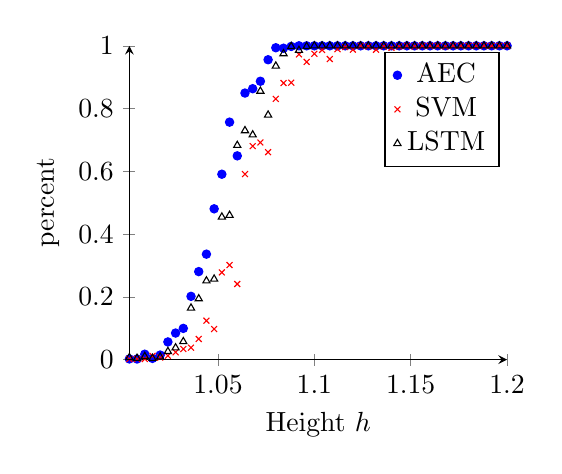
\begin{tikzpicture}
	\begin{axis}[
		xlabel={Height $h$},
		ylabel={percent},
		axis x line=bottom,
		axis y line=left,
		ymin=0,
		ymax=1,
scale=0.7
]
	\addplot[only marks, mark size=1.5, color=blue, mark=*] plot coordinates {
		(1.004, 0.00218818380744)
		(1.008, 0.002028397565923)
		(1.012, 0.017316017316017)
		(1.016, 0.004048582995951)
		(1.02, 0.014553014553015)
		(1.024, 0.056420233463035)
		(1.028, 0.084745762711864)
		(1.032, 0.099576271186441)
		(1.036, 0.201698513800425)
		(1.04, 0.28051391862955)
		(1.044, 0.336099585062241)
		(1.048, 0.480603448275862)
		(1.052, 0.590818363273453)
		(1.056, 0.756756756756757)
		(1.06, 0.649377593360996)
		(1.064, 0.849484536082474)
		(1.068, 0.863340563991323)
		(1.072, 0.887058823529412)
		(1.076, 0.955602536997886)
		(1.08, 0.993865030674847)
		(1.084, 0.992292870905588)
		(1.088, 0.998043052837573)
		(1.092, 1.0)
		(1.096, 1.0)
		(1.1, 1.0)
		(1.104, 1.0)
		(1.108, 1.0)
		(1.112, 1.0)
		(1.116, 1.0)
		(1.12, 1.0)
		(1.124, 1.0)
		(1.128, 1.0)
		(1.132, 1.0)
		(1.136, 1.0)
		(1.14, 1.0)
		(1.144, 1.0)
		(1.148, 1.0)
		(1.152, 1.0)
		(1.156, 1.0)
		(1.16, 1.0)
		(1.164, 1.0)
		(1.168, 1.0)
		(1.172, 1.0)
		(1.176, 1.0)
		(1.18, 1.0)
		(1.184, 1.0)
		(1.188, 1.0)
		(1.192, 1.0)
		(1.196, 1.0)
		(1.2, 1.0)
	};
	\addlegendentry{AEC}
	\addplot[only marks, mark size=1.5, color=red, mark=x] plot coordinates {
		(1.004, 0.00218818380744)
		(1.008, 0.002028397565923)
		(1.012, 0.002164502164502)
		(1.016, 0.012145748987854)
		(1.02, 0.006382978723404)
		(1.024, 0.012474012474013)
		(1.028, 0.023346303501946)
		(1.032, 0.033898305084746)
		(1.036, 0.038135593220339)
		(1.04, 0.065817409766454)
		(1.044, 0.124197002141328)
		(1.048, 0.097510373443983)
		(1.052, 0.27801724137931)
		(1.056, 0.301397205588822)
		(1.06, 0.240990990990991)
		(1.064, 0.591286307053942)
		(1.068, 0.680412371134021)
		(1.072, 0.691973969631236)
		(1.076, 0.661176470588235)
		(1.08, 0.830866807610994)
		(1.084, 0.881390593047035)
		(1.088, 0.882466281310212)
		(1.092, 0.972602739726027)
		(1.096, 0.948770491803279)
		(1.1, 0.974630021141649)
		(1.104, 0.986813186813187)
		(1.108, 0.957831325301205)
		(1.112, 0.989270386266094)
		(1.116, 0.995991983967936)
		(1.12, 0.987755102040816)
		(1.124, 1.0)
		(1.128, 0.997967479674797)
		(1.132, 0.987577639751553)
		(1.136, 0.998003992015968)
		(1.14, 0.993736951983299)
		(1.144, 0.997933884297521)
		(1.148, 1.0)
		(1.152, 0.997792494481236)
		(1.156, 1.0)
		(1.16, 1.0)
		(1.164, 1.0)
		(1.168, 0.997920997920998)
		(1.172, 1.0)
		(1.176, 1.0)
		(1.18, 1.0)
		(1.184, 1.0)
		(1.188, 1.0)
		(1.192, 1.0)
		(1.196, 1.0)
		(1.2, 1.0)
	};
	\addlegendentry{SVM}
	\addplot[only marks, mark size=1.5, color=black, mark=triangle] plot coordinates {
		(1.004, 0.006637168141593)
		(1.008, 0.004329004329004)
		(1.012, 0.01010101010101)
		(1.016, 0.004056795131846)
		(1.02, 0.008583690987124)
		(1.024, 0.026)
		(1.028, 0.03765690376569)
		(1.032, 0.057569296375267)
		(1.036, 0.164529914529915)
		(1.04, 0.194092827004219)
		(1.044, 0.251028806584362)
		(1.048, 0.256842105263158)
		(1.052, 0.454545454545455)
		(1.056, 0.460038986354776)
		(1.06, 0.682773109243697)
		(1.064, 0.72972972972973)
		(1.068, 0.716297786720322)
		(1.072, 0.85546875)
		(1.076, 0.779411764705882)
		(1.08, 0.935622317596567)
		(1.084, 0.975056689342404)
		(1.088, 0.99789029535865)
		(1.092, 0.985507246376812)
		(1.096, 0.99800796812749)
		(1.1, 1.0)
		(1.104, 1.0)
		(1.108, 1.0)
		(1.112, 1.0)
		(1.116, 1.0)
		(1.12, 1.0)
		(1.124, 1.0)
		(1.128, 1.0)
		(1.132, 1.0)
		(1.136, 1.0)
		(1.14, 1.0)
		(1.144, 1.0)
		(1.148, 1.0)
		(1.152, 1.0)
		(1.156, 1.0)
		(1.16, 1.0)
		(1.164, 1.0)
		(1.168, 1.0)
		(1.172, 1.0)
		(1.176, 1.0)
		(1.18, 1.0)
		(1.184, 1.0)
		(1.188, 1.0)
		(1.192, 1.0)
		(1.196, 1.0)
		(1.2, 1.0)
	};
	\addlegendentry{LSTM}
	\end{axis}
\end{tikzpicture}

		\subcaption{True-Positive rate}
\end{minipage}
\begin{minipage}[t]{0.45\textwidth}
		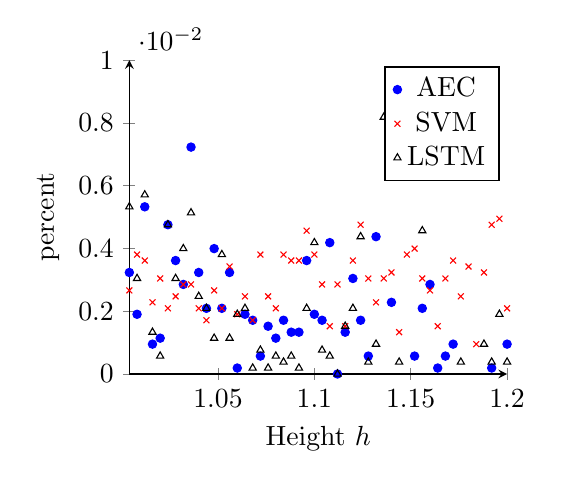
\begin{tikzpicture}
	\begin{axis}[
		xlabel={Height $h$},
		ylabel={percent},
		axis x line=bottom,
		axis y line=left,
		ymin=0,
		ymax=0.01,
scale=0.7
]
	\addplot[only marks, mark size=1.5, color=blue, mark=*] plot coordinates {
		(1.004, 0.003234398782344)
		(1.008, 0.001902587519026)
		(1.012, 0.005327245053272)
		(1.016, 0.000951293759513)
		(1.02, 0.001141552511416)
		(1.024, 0.004756468797565)
		(1.028, 0.003614916286149)
		(1.032, 0.002853881278539)
		(1.036, 0.007229832572298)
		(1.04, 0.003234398782344)
		(1.044, 0.002092846270928)
		(1.048, 0.003995433789954)
		(1.052, 0.002092846270928)
		(1.056, 0.003234398782344)
		(1.06, 0.000190258751903)
		(1.064, 0.001902587519026)
		(1.068, 0.001712328767123)
		(1.072, 0.000570776255708)
		(1.076, 0.001522070015221)
		(1.08, 0.001141552511416)
		(1.084, 0.001712328767123)
		(1.088, 0.001331811263318)
		(1.092, 0.001331811263318)
		(1.096, 0.003614916286149)
		(1.1, 0.001902587519026)
		(1.104, 0.001712328767123)
		(1.108, 0.004185692541857)
		(1.112, 0.0)
		(1.116, 0.001331811263318)
		(1.12, 0.003044140030441)
		(1.124, 0.001712328767123)
		(1.128, 0.000570776255708)
		(1.132, 0.00437595129376)
		(1.136, 0.010654490106545)
		(1.14, 0.002283105022831)
		(1.144, 0.015981735159817)
		(1.148, 0.012747336377473)
		(1.152, 0.000570776255708)
		(1.156, 0.002092846270928)
		(1.16, 0.002853881278539)
		(1.164, 0.000190258751903)
		(1.168, 0.000570776255708)
		(1.172, 0.000951293759513)
		(1.176, 0.011225266362253)
		(1.18, 0.021499238964992)
		(1.184, 0.015791476407915)
		(1.188, 0.018264840182648)
		(1.192, 0.000190258751903)
		(1.196, 0.011796042617961)
		(1.2, 0.000951293759513)
	};
	\addlegendentry{AEC}
	\addplot[only marks, mark size=1.5, color=red, mark=x] plot coordinates {
		(1.004, 0.002663622526636)
		(1.008, 0.003805175038052)
		(1.012, 0.003614916286149)
		(1.016, 0.002283105022831)
		(1.02, 0.003044140030441)
		(1.024, 0.002092846270928)
		(1.028, 0.002473363774734)
		(1.032, 0.002853881278539)
		(1.036, 0.002853881278539)
		(1.04, 0.002092846270928)
		(1.044, 0.001712328767123)
		(1.048, 0.002663622526636)
		(1.052, 0.002092846270928)
		(1.056, 0.003424657534247)
		(1.06, 0.001902587519026)
		(1.064, 0.002473363774734)
		(1.068, 0.001712328767123)
		(1.072, 0.003805175038052)
		(1.076, 0.002473363774734)
		(1.08, 0.002092846270928)
		(1.084, 0.003805175038052)
		(1.088, 0.003614916286149)
		(1.092, 0.003614916286149)
		(1.096, 0.004566210045662)
		(1.1, 0.003805175038052)
		(1.104, 0.002853881278539)
		(1.108, 0.001522070015221)
		(1.112, 0.002853881278539)
		(1.116, 0.001522070015221)
		(1.12, 0.003614916286149)
		(1.124, 0.004756468797565)
		(1.128, 0.003044140030441)
		(1.132, 0.002283105022831)
		(1.136, 0.003044140030441)
		(1.14, 0.003234398782344)
		(1.144, 0.001331811263318)
		(1.148, 0.003805175038052)
		(1.152, 0.003995433789954)
		(1.156, 0.003044140030441)
		(1.16, 0.002663622526636)
		(1.164, 0.001522070015221)
		(1.168, 0.003044140030441)
		(1.172, 0.003614916286149)
		(1.176, 0.002473363774734)
		(1.18, 0.003424657534247)
		(1.184, 0.000951293759513)
		(1.188, 0.003234398782344)
		(1.192, 0.004756468797565)
		(1.196, 0.004946727549467)
		(1.2, 0.002092846270928)
	};
	\addlegendentry{SVM}
	\addplot[only marks, mark size=1.5, color=black, mark=triangle] plot coordinates {
		(1.004, 0.005328258801142)
		(1.008, 0.003044719314938)
		(1.012, 0.005708848715509)
		(1.016, 0.001332064700285)
		(1.02, 0.000570884871551)
		(1.024, 0.004757373929591)
		(1.028, 0.003044719314938)
		(1.032, 0.003996194100856)
		(1.036, 0.005137963843958)
		(1.04, 0.002473834443387)
		(1.044, 0.00209324452902)
		(1.048, 0.001141769743102)
		(1.052, 0.003805899143673)
		(1.056, 0.001141769743102)
		(1.06, 0.001902949571836)
		(1.064, 0.00209324452902)
		(1.068, 0.000190294957184)
		(1.072, 0.000761179828735)
		(1.076, 0.000190294957184)
		(1.08, 0.000570884871551)
		(1.084, 0.000380589914367)
		(1.088, 0.000570884871551)
		(1.092, 0.000190294957184)
		(1.096, 0.00209324452902)
		(1.1, 0.00418648905804)
		(1.104, 0.000761179828735)
		(1.108, 0.000570884871551)
		(1.112, 0.0)
		(1.116, 0.001522359657469)
		(1.12, 0.00209324452902)
		(1.124, 0.004376784015224)
		(1.128, 0.000380589914367)
		(1.132, 0.000951474785918)
		(1.136, 0.008182683158896)
		(1.14, 0.016365366317793)
		(1.144, 0.000380589914367)
		(1.148, 0.006660323501427)
		(1.152, 0.007992388201713)
		(1.156, 0.004567078972407)
		(1.16, 0.01465271170314)
		(1.164, 0.007611798287345)
		(1.168, 0.01674595623216)
		(1.172, 0.008753568030447)
		(1.176, 0.000380589914367)
		(1.18, 0.013891531874405)
		(1.184, 0.026450999048525)
		(1.188, 0.000951474785918)
		(1.192, 0.000380589914367)
		(1.196, 0.001902949571836)
		(1.2, 0.000380589914367)
	};
	\addlegendentry{LSTM}
	\end{axis}
\end{tikzpicture}

		\subcaption{False-Positive rate}
\end{minipage}
\caption{Slight advantage for the \ac{aec} in the pulse detection}
\label{f:pulse}
\end{figure}
		
	\subsubsection{Sine Anomaly}
		The sine anomaly results are presented in figure \ref{f:sine}. The anomaly was detected best by the \ac{lstm} and worst by the \ac{svm}. This could imply that the \ac{svm} has trouble detecting values that oscillate around the expected values.\newline	
	The detection of 100\% with the \ac{lstm} as well as \ac{aec} is met at an amplitude of $a \approx \num{0.12}$. 

\begin{figure}[htb]
\centering
\begin{minipage}[t]{0.45\textwidth}
		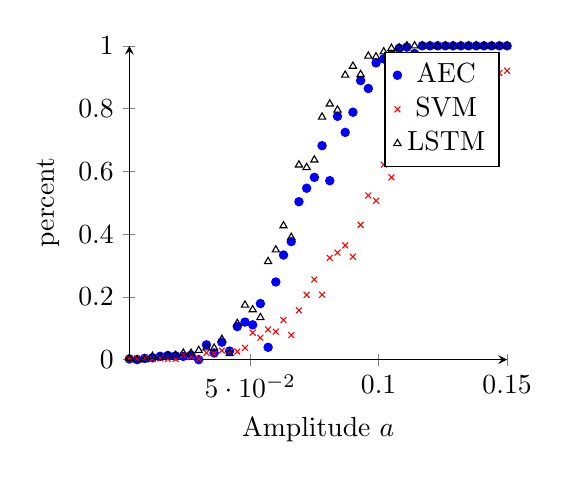
\begin{tikzpicture}
	\begin{axis}[
		xlabel={Amplitude $a$},
		ylabel={percent},
		axis x line=bottom,
		axis y line=left,
		ymin=0,
		ymax=1,
scale=0.7
]
	\addplot[only marks, mark size=1.5pt, color=blue, mark=*] plot coordinates {
		(0.003, 0.002079002079002)
		(0.006, 0.0)
		(0.009, 0.004089979550102)
		(0.012, 0.005825242718447)
		(0.015, 0.010729613733906)
		(0.018, 0.013215859030837)
		(0.021, 0.011976047904192)
		(0.024, 0.010504201680672)
		(0.027, 0.01417004048583)
		(0.03, 0.0)
		(0.033, 0.047210300429185)
		(0.036, 0.021413276231263)
		(0.039, 0.055670103092784)
		(0.042, 0.027426160337553)
		(0.045, 0.105376344086022)
		(0.048, 0.119733924611973)
		(0.051, 0.110878661087866)
		(0.054, 0.178640776699029)
		(0.057, 0.039301310043668)
		(0.06, 0.247464503042596)
		(0.063, 0.333333333333333)
		(0.066, 0.376321353065539)
		(0.069, 0.503225806451613)
		(0.072, 0.546168958742633)
		(0.075, 0.580851063829787)
		(0.078, 0.681818181818182)
		(0.081, 0.570247933884297)
		(0.084, 0.775377969762419)
		(0.087, 0.72421052631579)
		(0.09, 0.788381742738589)
		(0.093, 0.889370932754881)
		(0.096, 0.86405529953917)
		(0.099, 0.94560669456067)
		(0.102, 0.958419958419958)
		(0.105, 0.972746331236897)
		(0.108, 0.992277992277992)
		(0.111, 0.995859213250518)
		(0.114, 0.975659229208925)
		(0.117, 1.0)
		(0.12, 1.0)
		(0.123, 1.0)
		(0.126, 1.0)
		(0.129, 1.0)
		(0.132, 1.0)
		(0.135, 1.0)
		(0.138, 1.0)
		(0.141, 1.0)
		(0.144, 1.0)
		(0.147, 1.0)
		(0.15, 1.0)
	};
	\addlegendentry{AEC}
	\addplot[only marks, mark size=1.5pt, color=red, mark=x] plot coordinates {
		(0.003, 0.002079002079002)
		(0.006, 0.004106776180698)
		(0.009, 0.006134969325153)
		(0.012, 0.001941747572816)
		(0.015, 0.004291845493562)
		(0.018, 0.002202643171806)
		(0.021, 0.001996007984032)
		(0.024, 0.014705882352941)
		(0.027, 0.010121457489879)
		(0.03, 0.002252252252252)
		(0.033, 0.021459227467811)
		(0.036, 0.019271948608137)
		(0.039, 0.028865979381443)
		(0.042, 0.025316455696203)
		(0.045, 0.025806451612903)
		(0.048, 0.037694013303769)
		(0.051, 0.085774058577406)
		(0.054, 0.069902912621359)
		(0.057, 0.096069868995633)
		(0.06, 0.089249492900609)
		(0.063, 0.126068376068376)
		(0.066, 0.078224101479916)
		(0.069, 0.156989247311828)
		(0.072, 0.206286836935167)
		(0.075, 0.25531914893617)
		(0.078, 0.206818181818182)
		(0.081, 0.324380165289256)
		(0.084, 0.341252699784017)
		(0.087, 0.364210526315789)
		(0.09, 0.327800829875519)
		(0.093, 0.429501084598698)
		(0.096, 0.523041474654378)
		(0.099, 0.506276150627615)
		(0.102, 0.621621621621622)
		(0.105, 0.580712788259958)
		(0.108, 0.642857142857143)
		(0.111, 0.652173913043478)
		(0.114, 0.789046653144016)
		(0.117, 0.708074534161491)
		(0.12, 0.748936170212766)
		(0.123, 0.805168986083499)
		(0.126, 0.869120654396728)
		(0.129, 0.837310195227766)
		(0.132, 0.852008456659619)
		(0.135, 0.885714285714286)
		(0.138, 0.922222222222222)
		(0.141, 0.877637130801688)
		(0.144, 0.896341463414634)
		(0.147, 0.91358024691358)
		(0.15, 0.920600858369099)
	};
	\addlegendentry{SVM}
	\addplot[only marks, mark size=1.5pt, color=black, mark=triangle] plot coordinates {
		(0.003, 0.004149377593361)
		(0.006, 0.0)
		(0.009, 0.0)
		(0.012, 0.010660980810235)
		(0.015, 0.006550218340611)
		(0.018, 0.012738853503185)
		(0.021, 0.013670119565316)
		(0.024, 0.02102908334352)
		(0.027, 0.020790020790021)
		(0.03, 0.029319313183855)
		(0.033, 0.037848605577689)
		(0.036, 0.036964980544747)
		(0.039, 0.064777327935223)
		(0.042, 0.019230769230769)
		(0.045, 0.115537848605578)
		(0.048, 0.174)
		(0.051, 0.159090909090909)
		(0.054, 0.133891213389121)
		(0.057, 0.312625250501002)
		(0.06, 0.349896480331263)
		(0.063, 0.426724137931034)
		(0.066, 0.389690721649485)
		(0.069, 0.620481927710843)
		(0.072, 0.612284069097889)
		(0.075, 0.636363636363636)
		(0.078, 0.773127753303965)
		(0.081, 0.814893617021277)
		(0.084, 0.795501022494888)
		(0.087, 0.906693711967546)
		(0.09, 0.935146443514644)
		(0.093, 0.908713692946058)
		(0.096, 0.967280163599182)
		(0.099, 0.964948453608247)
		(0.102, 0.980891719745223)
		(0.105, 0.992263056092843)
		(0.108, 0.993534482758621)
		(0.111, 1.0)
		(0.114, 1.0)
		(0.117, 1.0)
		(0.12, 1.0)
		(0.123, 1.0)
		(0.126, 1.0)
		(0.129, 1.0)
		(0.132, 1.0)
		(0.135, 1.0)
		(0.138, 1.0)
		(0.141, 1.0)
		(0.144, 1.0)
		(0.147, 1.0)
		(0.15, 1.0)
	};
	\addlegendentry{LSTM}
	\end{axis}
\end{tikzpicture}

		\subcaption{True-Positive rate}
\end{minipage}
\begin{minipage}[t]{0.45\textwidth}
		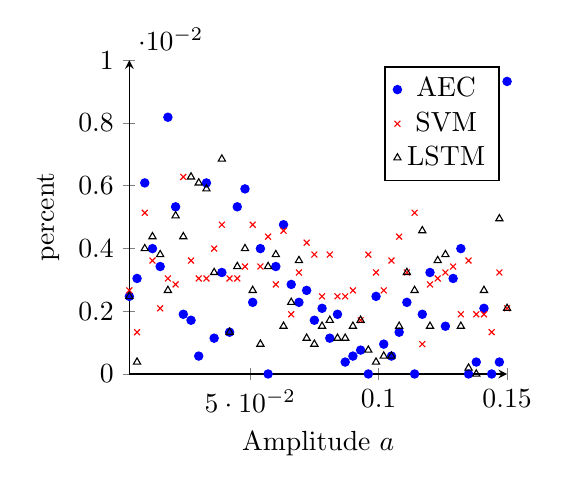
\begin{tikzpicture}
	\begin{axis}[
		xlabel={Amplitude $a$},
		ylabel={percent},
		axis x line=bottom,
		axis y line=left,
		ymin=0,
		ymax=0.01,
scale=0.7
]
	\addplot[only marks, mark size=1.5, color=blue, mark=*] plot coordinates {
		(0.003, 0.002473363774734)
		(0.006, 0.003044140030441)
		(0.009, 0.006088280060883)
		(0.012, 0.003995433789954)
		(0.015, 0.003424657534247)
		(0.018, 0.008181126331811)
		(0.021, 0.005327245053272)
		(0.024, 0.001902587519026)
		(0.027, 0.001712328767123)
		(0.03, 0.000570776255708)
		(0.033, 0.006088280060883)
		(0.036, 0.001141552511416)
		(0.039, 0.003234398782344)
		(0.042, 0.001331811263318)
		(0.045, 0.005327245053272)
		(0.048, 0.00589802130898)
		(0.051, 0.002283105022831)
		(0.054, 0.003995433789954)
		(0.057, 0.0)
		(0.06, 0.003424657534247)
		(0.063, 0.004756468797565)
		(0.066, 0.002853881278539)
		(0.069, 0.002283105022831)
		(0.072, 0.002663622526636)
		(0.075, 0.001712328767123)
		(0.078, 0.002092846270928)
		(0.081, 0.001141552511416)
		(0.084, 0.001902587519026)
		(0.087, 0.000380517503805)
		(0.09, 0.000570776255708)
		(0.093, 0.00076103500761)
		(0.096, 0.0)
		(0.099, 0.002473363774734)
		(0.102, 0.000951293759513)
		(0.105, 0.000570776255708)
		(0.108, 0.001331811263318)
		(0.111, 0.002283105022831)
		(0.114, 0.0)
		(0.117, 0.001902587519026)
		(0.12, 0.003234398782344)
		(0.123, 0.006468797564688)
		(0.126, 0.001522070015221)
		(0.129, 0.003044140030441)
		(0.132, 0.003995433789954)
		(0.135, 0.0)
		(0.138, 0.000380517503805)
		(0.141, 0.002092846270928)
		(0.144, 0.0)
		(0.147, 0.000380517503805)
		(0.15, 0.009322678843227)
	};
	\addlegendentry{AEC}
	\addplot[only marks, mark size=1.5, color=red, mark=x] plot coordinates {
		(0.003, 0.002663622526636)
		(0.006, 0.001331811263318)
		(0.009, 0.00513698630137)
		(0.012, 0.003614916286149)
		(0.015, 0.002092846270928)
		(0.018, 0.003044140030441)
		(0.021, 0.002853881278539)
		(0.024, 0.006278538812785)
		(0.027, 0.003614916286149)
		(0.03, 0.003044140030441)
		(0.033, 0.003044140030441)
		(0.036, 0.003995433789954)
		(0.039, 0.004756468797565)
		(0.042, 0.003044140030441)
		(0.045, 0.003044140030441)
		(0.048, 0.003424657534247)
		(0.051, 0.004756468797565)
		(0.054, 0.003424657534247)
		(0.057, 0.00437595129376)
		(0.06, 0.002853881278539)
		(0.063, 0.004566210045662)
		(0.066, 0.001902587519026)
		(0.069, 0.003234398782344)
		(0.072, 0.004185692541857)
		(0.075, 0.003805175038052)
		(0.078, 0.002473363774734)
		(0.081, 0.003805175038052)
		(0.084, 0.002473363774734)
		(0.087, 0.002473363774734)
		(0.09, 0.002663622526636)
		(0.093, 0.001712328767123)
		(0.096, 0.003805175038052)
		(0.099, 0.003234398782344)
		(0.102, 0.002663622526636)
		(0.105, 0.003614916286149)
		(0.108, 0.00437595129376)
		(0.111, 0.003234398782344)
		(0.114, 0.00513698630137)
		(0.117, 0.000951293759513)
		(0.12, 0.002853881278539)
		(0.123, 0.003044140030441)
		(0.126, 0.003234398782344)
		(0.129, 0.003424657534247)
		(0.132, 0.001902587519026)
		(0.135, 0.003614916286149)
		(0.138, 0.001902587519026)
		(0.141, 0.001902587519026)
		(0.144, 0.001331811263318)
		(0.147, 0.003234398782344)
		(0.15, 0.002092846270928)
	};
	\addlegendentry{SVM}
	\addplot[only marks, mark size=1.5, color=black, mark=triangle] plot coordinates {
		(0.003, 0.002473834443387)
		(0.006, 0.000380589914367)
		(0.009, 0.003996194100856)
		(0.012, 0.004376784015224)
		(0.015, 0.003805899143673)
		(0.018, 0.002664129400571)
		(0.021, 0.005042816365366)
		(0.024, 0.004376784015224)
		(0.027, 0.00627973358706)
		(0.03, 0.006089438629876)
		(0.033, 0.005899143672693)
		(0.036, 0.003235014272122)
		(0.039, 0.006850618458611)
		(0.042, 0.001332064700285)
		(0.045, 0.003425309229305)
		(0.048, 0.003996194100856)
		(0.051, 0.002664129400571)
		(0.054, 0.000951474785918)
		(0.057, 0.003425309229305)
		(0.06, 0.003805899143673)
		(0.063, 0.001522359657469)
		(0.066, 0.002283539486204)
		(0.069, 0.003615604186489)
		(0.072, 0.001141769743102)
		(0.075, 0.000951474785918)
		(0.078, 0.001522359657469)
		(0.081, 0.001712654614653)
		(0.084, 0.001141769743102)
		(0.087, 0.001141769743102)
		(0.09, 0.001522359657469)
		(0.093, 0.001712654614653)
		(0.096, 0.000761179828735)
		(0.099, 0.000380589914367)
		(0.102, 0.000570884871551)
		(0.105, 0.000570884871551)
		(0.108, 0.001522359657469)
		(0.111, 0.003235014272122)
		(0.114, 0.002664129400571)
		(0.117, 0.004567078972407)
		(0.12, 0.001522359657469)
		(0.123, 0.003615604186489)
		(0.126, 0.003805899143673)
		(0.129, 0.008943862987631)
		(0.132, 0.001522359657469)
		(0.135, 0.000190294957184)
		(0.138, 0.0)
		(0.141, 0.002664129400571)
		(0.144, 0.006850618458611)
		(0.147, 0.004947668886775)
		(0.15, 0.002092846270928)
	};
	\addlegendentry{LSTM}
	\end{axis}
\end{tikzpicture}

		\subcaption{False-Positive rate}
\end{minipage}
\caption{\ac{aec} and \ac{lstm} are almost equal whereas the \ac{svm} has quite some detection problems}
\label{f:sine}
\end{figure}

\chapter{Machine Learning Model Workflow - Creating a Framework}
To train, convert, upload and finally execute a model, a framework to define these steps is needed. In figure \ref{f:model_framework} a general concept of the corresponding workflow is shown. The ground and space segment are separated. They communicate and transfer the model via the \acf{pus} standard \cite{pus}. \newline
For simplification, the handling of models on ground as well as on board is only considered with the use of the Tensorflow library. But ultimately, a framework should support multiple machine learning libraries.

In the following a rough idea of a framework with the example of a tf-lite model will be discussed. The presented framework is being development by the software group from DLR Bremen. \newline
The discussion hereby is lead by the workflow. Starting from model creation and training, to serializing the model for transmission and finally to executing the uploaded model in a specified application.

\begin{figure}[htb]
\centering
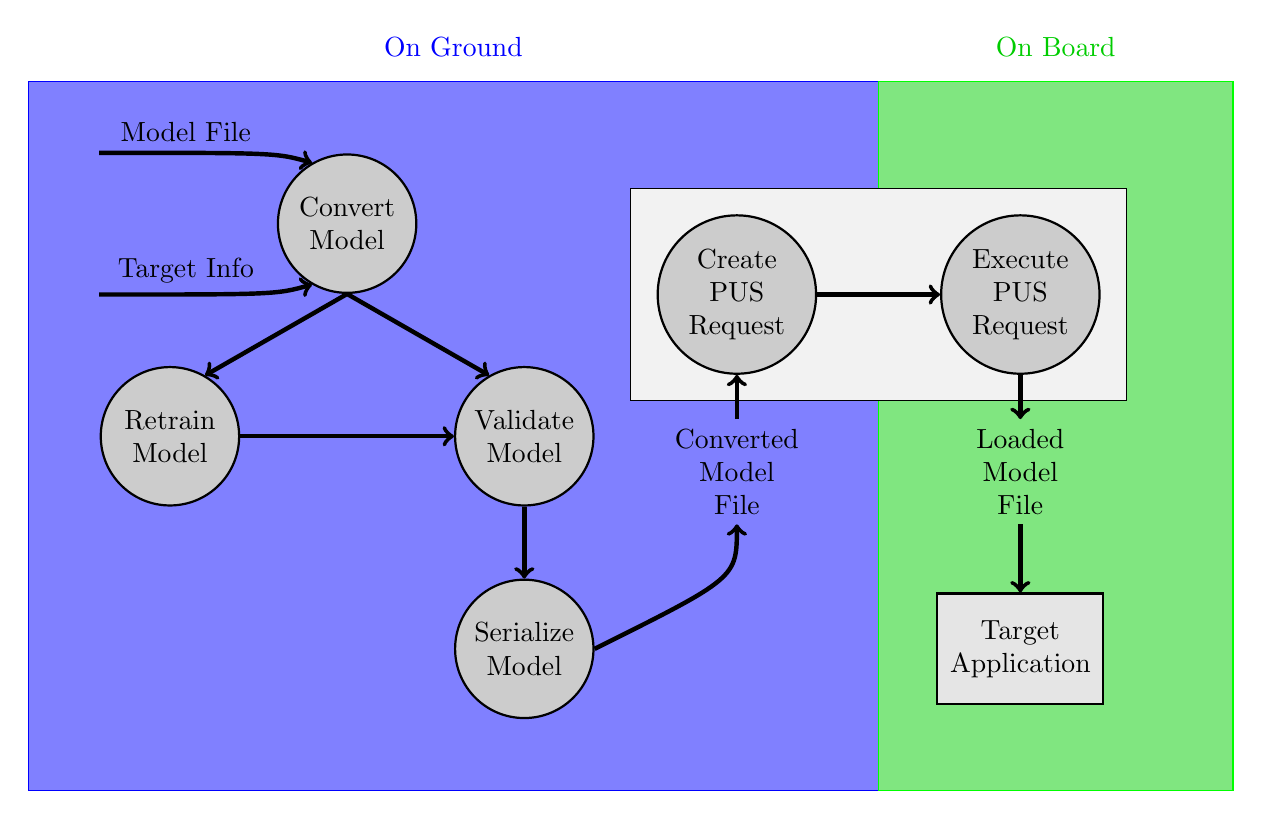
\begin{tikzpicture}[
	block/.style={
		circle,
		minimum size=5em,
		draw=black,
		thick,
		fill=black!20,
		align=center,
	},
	scale=0.9
]

\draw[color=blue, fill=blue!50] (-6,-5) rectangle (6,5);
\node[align=center,color=blue] at (0, 5.5) {On Ground};
\draw[color=green, fill=black!20!green!50] (6,-5) rectangle (11,5);
\node[align=center,color=black!20!green] at (8.5, 5.5) {On Board};

\draw[color=black, fill=black!5] (2.5,0.5) rectangle (9.5,3.5);

\node[block] (cm) at (-1.5,3) {Convert\\ Model};

\node[block] (rm) at (-4,0) {Retrain\\ Model};
\node[block] (vm) at (1,0) {Validate\\ Model};

\node[block] (sm) at (1,-3) {Serialize\\ Model};

\draw[->,ultra thick] (cm.south) -- (rm.60);
\draw[->,ultra thick] (cm.south) -- (vm.120);
\draw[->,ultra thick] (rm.east) -- (vm.west);
\draw[->,ultra thick] (vm.south) -- (sm.north);

\draw[->,ultra thick] (-5,4) .. node[pos=0.2, above] {Model File} controls (-2.5,4) .. (cm.120);
\draw[->,ultra thick] (-5,2) .. node[pos=0.2, above] {Target Info} controls (-2.5,2) .. (cm.240);

\node[block] (gpr) at (4,2) {Create\\ PUS\\ Request};
\node[align=center] (cmf) at (4,-0.5) {Converted\\ Model\\ File};
\draw[->,ultra thick] (sm.east) .. controls (4,-2) .. (cmf.south);
\draw[->,ultra thick] (cmf.north) -- (gpr.south);

\node[block] (epr) at (8,2) {Execute\\ PUS\\ Request};
\draw[->,ultra thick] (gpr.east) -- (epr.west);

\node[align=center] (lmf) at (8,-0.5) {Loaded\\ Model\\ File};
\node[align=center,thick,rectangle,draw=black,fill=black!10, minimum width=6em, minimum height=4em] (ta) at (8,-3) {Target\\ Application};

\draw[->,ultra thick] (epr.south) -- (lmf.north);
\draw[->,ultra thick] (lmf.south) -- (ta.north);

\end{tikzpicture}

\caption{Model Training, Transfer and Execution Framework.}
\label{f:model_framework}
\end{figure}

\section{Ground Training and Serialization}
Essentially, a framework should enable the creation of models in various ways with different libraries. This model file would need to be translated to a more general format, to be able to retrain with new data and to validate it. But with Tensorflow one can skip this step for now and lay the focus not on different architectures and libraries, but on handling the model itself. \newline
This means, a model needs to be trained with existing data, then validated and finally serialized. In the chapter before the training and validation of different Tensorflow models was already shown. The next step here is to serialize the model, to fit it into a machine readable byte array, which can be uploaded via telecommands onto a satellite.

The small, serialized format in Tensorflow is the so called \enquote{flatbuffer}. The flatbuffer only contains the most necessary information about the converted neural network. This includes only the structure and weights. \newline
To convert a neural network, it first has to be converted to a tf-lite model in an intermediate step. Unfortunately in Tensorflow Lite, not all kinds of neural networks are fully supported yet. The \acp{rnn} for example are still in an experimental state, hence the discussed \ac{lstm} will not be considered fully usable.

\section{Transfer and Upload}
The size of the converted neural network is rather small, in terms of storage. This can make updates rather easy. The \ac{pus} standard allows for a maximum package data size of $\SI{65535}{\byte}$. The tf-lite models created in the previous chapter did range from $\SI{10}{\kilo\byte}$ to $\SI{1}{\mega\byte}$. In the best case, the model is small enough to be uploaded within one package. In the worst case a model would need numerous consecutive packages. 

In the framework, this prerequisite helps to propose an additional \ac{pus} service for utilization of tf-lite models and machine learnings applications. This service has then the task to manage new models, model updates and the deletion of outdated models. A second task is to make these models available for other applications on board of the satellite.

\section{On-Board Execution}
For the model execution, a specific application has to be written. This application has to first verify the flatbuffer to prevent the execution of a corrupted model. The flatbuffer can verified once it is loaded into the memory. Then can be fed with new incoming data and executed to predict anomalies in the data.

The application on board of the \ac{spc} will be written in C/C++ as this corresponds to the language of the Tensorflow library and the flight software.

\chapter{Implementation of the Framework - Demonstration}
The implementation will be done as a proof-of-concept and therefore kept minimalistic. The implementation includes the export of a Tensorflow model written in Python and the import and execution on an embedded system serving as demonstrator. The transfer will be excluded as this is already defined by various standards (e.g. \cite{spp}). 

This chapter will lead through the entire building process of a complete demonstrator. \newline
First the export and serialization of the model are demonstrated. In a second step the model has to be executed on a demonstration board running an embedded system. For that, the Tensorflow sources have to be cross-compiled to match the target system. Therefore the setup of a cross-compiler will be described as necessary prerequisite.

\section{Model Export}
To export and save a model in Python, only two steps are needed. The first step is to convert the model to a tf-lite model with the help of the \textit{TFLiteConverter}. The second step is the export itself.

The conversion to a tf-lite model can happen on the basis of a saved model or a model built with either Tensorflow or Keras\footnote{Keras is an API built on top of Tensorflow and offers a more powerful framework}\cite{keras}. A typical conversion and export would look like the following example:

\newpage
\begin{lstlisting}[caption={model export}, language=python]
# Convert the model
converter = tf.lite.TFLiteConverter.from_keras_model(model)
tflite_model = converter.convert()

# Save the model
with open('model.tflite', 'wb') as f:
  f.write(tflite_model)
\end{lstlisting}

For models containing \acp{rnn} (like the \ac{lstm}) an additional conversion step is necessary, which will not be further investigated here.

\section{Tensorflow Cross-Compilation}
For cross-compilation an extra toolchain is needed. There are two options, either to take a pre-made toolchain or to forge a custom one. Here the decision was made for the latter. \newline
The advantage of a custom toolchain is, that the whole compilation process can be completely understood. This helps in case of required modifications. Second, the modifications themselves are much easier to implement. And third, with understanding the build-process, there is also much more control of how the sources are compiled.

In the following a custom toolchain for an ARM processor will be set up with the basic libraries. Once that is done, the Tensorflow sources will be compiled. With the complete toolchain set up, a simple program to load Tensorflow models in C++ on a demonstration board will be presented.

\subsection{ARM Toolchain}
For the toolchain the GNU compiler collection (\textit{gcc}) will be used. The toolchain will be solely based on the packages provided by the gnu project \cite{gnu-proj}. The only exception is the modified linux kernel which has been taken from Analog Devices Inc. The platform for working and compiling is a debian linux system hosted on a docker container. 

For the cross-compiler to work, the necessary steps are to first build the \textit{binutils} and configure the \textit{linux headers}. With this at hand, the \textit{gcc} can be boostraped. Once the \textit{gcc} is partially compiled, the \textit{glibc} can also be partially compiled. With these partial \textit{glibc} the \textit{gcc} can be fully compiled and then be used to finalize the \textit{glibc}. A list of the used packages with concrete versions can be found in table \ref{t:software}.

Once the compiler and the libraries are ready, the basic toolchain is set up and can be used for further cross-compilation.

\begin{table}[htb]
\centering
\caption{Used sources for the cross-compilation.}
\begin{tabular}{lll}
\toprule
Package			& Version	& Source \\ \midrule
GCC				& 8.4.0 	& \url{gnu.org/software/gcc} \\
Binutils		& 2.32 		& \url{gnu.org/software/binutils} \\
GLIBC			& 2.28		& \url{gnu.org/software/libc} \\
Linux Headers	& 4.9		& \url{github.com/analogdevicesinc/linux} \\
\bottomrule
\end{tabular}
\label{t:software}
\end{table}

\subsection{Compiling Tensorflow Sources}
Now the Tensorflow sources can be compiled to generate a usable library. For that, the corresponding source files are cloned from the git, modified and then run against the toolchain from the section before.

\paragraph*{Sources} \hfill

First the Tensorflow files in the version \textbf{r2.4} need to be downloaded:

\begin{lstlisting}[caption={git clone}, language=bash]
$ git clone https://github.com/tensorflow/tensorflow
$ cd tensorflow
$ git checkout r2.4
\end{lstlisting}

\paragraph*{Dependencies} \hfill

The next step is to download the required dependencies:

\begin{lstlisting}[caption={dependencies}, language=bash]
$ ./tensorflow/tensorflow/lite/tools/make\
	/download_dependencies.sh
\end{lstlisting}

\paragraph*{Modifications} \hfill

To make the cross-compilation with ARM work, three files have to be modified. First the build script, second the \textit{Makefile} and third the \textit{util.cpp} file. Starting with the build script (\textit{./tensorflow/tensorflow/lite/tools/make/build\_aarch64\_lib.sh}):

\begin{lstlisting}[caption={build\_aarch64\_lib.sh}, language=bash]
[31] make -j ${NO_JOB} TARGET=arm -C "${TENSORFLOW_DIR}"\
	-f tensorflow/lite/tools/make/Makefile $@
\end{lstlisting}

this can be saved as \textit{build\_arm\_lib.sh}.

Next step is the \textit{Makefile} (\textit{./tensorflow/tensorflow/lite/tools/make/Makefile}):

\begin{lstlisting}[caption={Makefile}, language=make]
[51] INCLUDES += -I/home/dlr/arm/opt\
	/arm-linux-gnueabihf/include
...
[61] -ldl \
[62] -latomic
...
[70] LDOPTS := -L/home/dlr/arm/opt/arm-linux-gnueabihf/lib
...
[72] TARGET_TOOLCHAIN_PREFIX := arm-linux-gnueabihf-
\end{lstlisting}

And at last, one minor change has to made to the source file \textit{util.cpp} (\textit{./tensorflow/tensorflow/lite/tools/make/downloads/flatbuffers/src/util.cpp}):

\begin{lstlisting}[caption={util.cpp}, language=c++]
[36] -- #  include <limits.h>
[36] ++ #  include <linux/limits.h>
\end{lstlisting}

\paragraph*{Final building step} \hfill

Now the build script can be started:

\begin{lstlisting}[caption={build\_arm\_lib.sh}, language=bash]
$ ./tensorflow/tensorflow/lite/tools/make/build_arm_lib.sh
\end{lstlisting}

In the end, a library is generated which will be used for the projects. The library is located in \textit{tensorflow/tensorflow/lite/make/gen/arm\_x86\_64/lib/libtensorflow-lite.a}.

%\paragraph*{Note:} There is also an experimental approach in tensorflow with CMake where only an additional toolchain definition file has to be generated. This approach has not been tested by the author.

\subsection{Makefile for Custom Projects}
Now that the ARM cross-compilation toolchain and Tensorflow libraries are both set up, they can be used to create and compile custom projects. The Makefile in listing \ref{l:make} shows only the most important configurations to use tensorflow. In the \textit{LIBFLAGS} the search destination for the tensorflow library is given, in this case it will be in the same directory as the Makefile itself. The tf-lite library is then specified within the \textit{LDFLAGS}. At last, the header file location needs to be set. In the case of the minimal example provided by Tensorflow, only the standard Tensorflow headers and the flatbuffers are needed. 

This configuration will then be used for the model import in the next section.

\begin{lstlisting}[caption={Makefile}, language=make, label={l:make}]
LIBFLAGS := -L./
LDFLAGS := -lstdc++ \
-lpthread \
-lm \
-ldl \
-lz \
-latomic \
-ltensorflow-lite

INC_DIRS := $(shell find $(SRC_DIRS) -type d) \
../tensorflow \
../tensorflow/tensorflow/lite/tools/make/\
	downloads/flatbuffers/include
\end{lstlisting}

\section{Model Import and Execution in C++}
To import the model and execute the neural network within, a short program in C++ is written. This program loads the tf-lite model in its serialized form as a flatbuffer and performs some checks. If the model turns out to be valid the input data can be fed in. 

As a demonstration and performance evaluation, the three neural networks presented in chapter \ref{c:selection} with the same datasets were tested on an evaluation board. \newline
In the case of the \ac{aec}, the only calculation the neural network does is the compression and decompression of the input data. Hence the comparison of these two data vectors (input and ouput) have to be done in the program. \newline
In the listing \ref{l:cpp} the code to demonstrate the functionality of the model is written. To increase readability of the code, the necessary checks are not shown.

\begin{lstlisting}[caption={model-load}, language=c++, label={l:cpp}]
#include <cstdio>
#include "tensorflow/lite/interpreter.h"
#include "tensorflow/lite/kernels/register.h"
#include "tensorflow/lite/model.h"
#include "tensorflow/lite/optional_debug_tools.h"

size_t load_data_from_file(const char * filename,
 float buffer[]);
void interfere_model(std::unique_ptr<tflite::Interpreter> 
 &interpreter, float buffer[], size_t length);
bool check_result((std::unique_ptr<tflite::Interpreter> 
 &interpreter, float boundary);

int main(int argc, char* argv[]) {
 const char* model_file = argv[1];
 const char* data_file = argv[2];

 // Load model
 std::unique_ptr<tflite::FlatBufferModel> model =
  tflite::FlatBufferModel::BuildFromFile(filename);
	
 // Build the interpreter to read the model
 tflite::ops::builtin::BuiltinOpResolver resolver;
 tflite::InterpreterBuilder builder(*model, resolver);
 std::unique_ptr<tflite::Interpreter> interpreter;
 builder(&interpreter);
  
 // Allocate tensor buffers.
 interpreter->AllocateTensors();
 tflite::PrintInterpreterState(interpreter.get());

 // Interfere model (interpreter->Invoke())
 float buffer[5256*100];
 size_t length = load_data_from_file(data_file, buffer);
 infere_model(interpreter, buffer, length);

 return 0;
}
\end{lstlisting}

The evaluation board consists of an ARM Cortex-A9 core with a frequency of $\SI{1}{\giga\hertz}$ and it has $\SI{1}{\giga\byte}$ of RAM. \newline
In table \ref{t:performance} the needed clock cycles for execution of these models are listed. The performance was only measured for the interference of the model and the evaluation, not for the model allocation and not for loading the datasets.

\begin{table}[htb]
\centering
\caption{Performance measurement of the three models presented in chapter \ref{c:selection}}
\label{t:performance}
\begin{tabular}{lllll}
\toprule
Model		& Total Params	& Trainable Params	& Clock Cycles		& Seconds \\ \midrule
\ac{aec}	& $\num{5125}$	& $\num{5125}$		& $\num{344e3}$	& $\num{0.344}$ \\
\ac{lstm}	& $\num{6300}$	& $\num{6300}$		& $\num{134e6}$	& $\num{134}$ \\
\ac{svm}	& $\num{210947}$ & $\num{4099}$	& $\num{785e4}$	& $\num{7.6}$ \\
\bottomrule
\end{tabular}
\end{table}

%\chapter{Validation}

Warum muss es validiert werden?

Wie können wir das validieren?

Analytisch versus Empirisch
%% End of Inclusion %%%

\chapter{Conclusion}

In this project it was shown, that more sophisticated techniques for spacecraft data analysis are needed and that this demand can be matched with machine learning techniques including neural networks. The possible solutions involved \acfp{aec}, \acfp{svm} and \acfp{lstm} provided by the Tensorflow library \cite{tf-web}.\newline
In a further analysis these three types of networks were discussed and compared. And they did prove to be able to detect contextual anomalies with feasible effort.

The \ac{aec} did show to be the most cost-effective solution for simple and repetitive data. Whereas the \ac{lstm} infers a higher computational load, that might, however, lead to the detection of more complex anomalies that are beyond the scope of this study. The highest computational load was induced by the \ac{svm}, which was always behind regarding detection rates.

As the neural networks proved to be effective in detecting anomalies, a framework for providing these techniques on board of a satellite was developed. \newline
The framework did define the steps of converting the machine learning model to a serialized version for the upload from ground to space. The upload management was set to be done via the \acf{pus} standard. On board the execution was defined to be handed over to a specific application.

The workflow was then demonstrated as proof-of-concept on an evaluation board with an ARM processor. The demonstration did show the way from the development of the machine learning model till the execution on the evaluation board. \newline
This did prove to be a feasible and effective way of implementing autonomous anomaly detection on board of a spacecraft.

\renewcommand\cleardoublepage{%
 \clearpage
 \ifodd\value{page}\else\stepcounter{page}\fi
}

\appendix

\bibliographystyle{unsrtdin} %gerdipl} %unsrt %gerdipl
\bibliography{Appendix/books} % BIB-Datei mit Literatur


\chapter{Source Code}

\section{Auto-Encoder}
\label{c:src_aec}
\begin{lstlisting}[caption={Auto-Encoder}, language=python]
aec = tf.keras.Sequential(tf.keras.Input(shape=(datasize,)),
 tf.keras.layers.Dense(units=25, activation="tanh"),
 tf.keras.layers.Dense(units=datasize, 
  activation="sigmoid"),])
\end{lstlisting}

\section{Long Short-Term Memory}
\label{c:src_lstm}
\begin{lstlisting}[caption={Long Short-Term Memory}, language=python]
lstm = tf.keras.Sequential(tf.keras.Embedding
  (10, 10, input_length=datasize),
 tf.keras.LSTM(1),
 tf.keras.layers.Dense(units=datasize, activation="tanh"),])
\end{lstlisting}

\newpage
\section{Support Vector Machine}
\label{c:src_svm}
\begin{lstlisting}[caption={Support Vector Machine}, language=python]
svm = tf.keras.Sequential(tf.keras.Input(shape=(datasize,)),
 tf.keras.layers.experimental.RandomFourierFeatures(
  output_dim=2048, kernel_initializer="laplacian", 
  trainable=True),
 tf.keras.layers.Dense(units=2, activation="sigmoid"),])
\end{lstlisting}

%
\begin{thebibliography}{9}
\bibitem{handbook}
Wilfried Ley, Klaus Wittmann, Willi Hallmann.
\textit{Handbook of Space Technology}
Wiley, 2009

\bibitem{athmos} 
Corey O'Meara, Leonard Schlag, Luisa Faltenbacher and Martin Wickler.
\textit{ATHMoS: Automated Telemetry Health Monitoring System at GSOC using Outlier Detection and Supervised Machine Learning}. 
German Aerospace Center, Wessling, Germany

\bibitem{aiforspace} 
Jan-Gerd Meß, Frank Dannemann and Fabian Greif.
\textit{Techniques of Artificial Intelligence for Space Applications - A Survey}. 
Conference Paper, February 2019

\bibitem{pus} 
European Cooperation for Space Standardization
\textit{Telemetry and telecommand packet utilization}. 
ECSS-E-ST-70-41C, April 2016

\end{thebibliography}

\end{document}